%----------------------------------------------------------------------------
%Type of document
\documentclass{beamer}

%----------------------------------------------------------------------------
%Packages
\usepackage{amsmath}
\usepackage{hyperref}
\usepackage{subfigure}
\usepackage{graphicx}
\usepackage{centernot}
\usepackage{appendixnumberbeamer}

%----------------------------------------------------------------------------
%Local adjustments of settings and definitions
\setcounter{MaxMatrixCols}{10}
\setbeamertemplate{caption}[numbered]
\definecolor{links}{HTML}{2A1B81}
\hypersetup{colorlinks,linkcolor=,urlcolor=links}

%----------------------------------------------------------------------------
%Beamer theme (Madrid and Frankfurt are good options)
\usetheme{Madrid}

%----------------------------------------------------------------------------
%Start document
\begin{document}

%----------------------------------------------------------------------------
%Front matter
\title[Financial Frictions and Crises]{Financial Frictions and Crises}
\author[Bidder]{Rhys Bidder}
\institute[FRBSF]{Federal Reserve Bank of San Francisco}
\date{Michaelmas Term 2019}
\maketitle

%----------------------------------------------------------------------------
%Main body

\begin{frame}{Disclaimer}

The views expressed in this presentation, and all errors and omissions, should be regarded as those solely of the authors, and are not necessarily those of the Federal Reserve Bank of San Francisco, the Federal Reserve Board of Governors or the Federal Reserve System.

\end{frame}

%-------------------------------------------------------
\section{The Importance of Capital}
%-------------------------------------------------------

\begin{frame}

\begin{center}
{\LARGE The Importance of Capital}
\end{center}

\end{frame}

%-------------------------------------------------------

%-------------------------------------------------------

\begin{frame}{Firm balance sheet}

A firm's balance sheet has two sides
	\begin{itemize}
	\item	Assets: Cash, intellectual property, inventory, receivables, machinery, trucks, real estate\ldots
	\item	Liabilities: Bank loans, commercial paper, trade credit, long term debt/bonds, capital
	\end{itemize}
\vspace{2mm}
If a firm's assets $>$ liabilities (\emph{excluding capital}) then we say it is `solvent'
	\begin{itemize}
	\item	Capital $\approx$ buffer of asset value over obligations to \textit{external creditors}
	\item	Simplifying somewhat, it comprises equity and retained earnings
	\item	Natural to think of it as liabilities \textit{to the bank's owners} (shareholders)
	\end{itemize}

\end{frame}

%-------------------------------------------------------

%-------------------------------------------------------

\begin{frame}{Bank balance sheet}

A \textbf{bank} balance sheet also has two sides
	\begin{itemize}
	\item	Assets: Traditionally predominantly loans (also securities, cash etc.)
	\item	Liabilities: Deposits, wholesale funding, bonds, \textbf{capital}
	\end{itemize}
\vspace{2mm}
Other than the composition of the balance sheet, the essential logic of a bank balance sheet is the same as in the firm case
	\begin{itemize}
	\item	The `other than' is obviously very important!
	\end{itemize} 
\vspace{2mm}
Confusing terminology: People (and I will) often refer to the bank's liabilities as excluding equity
	\begin{itemize}
	\item	Under this relabeling\ldots
	\vspace{1mm}
	\item[]	\centering \textcolor{red}{solvency $\Leftrightarrow$ (assets $\geq$ `liabilities') $\Leftrightarrow$ capital $>0$}
	\end{itemize}

\end{frame}

%-------------------------------------------------------

%-------------------------------------------------------

\begin{frame}{Bank balance sheet}

\begin{figure}
\begin{center}

\resizebox{0.30\textwidth}{!}{%
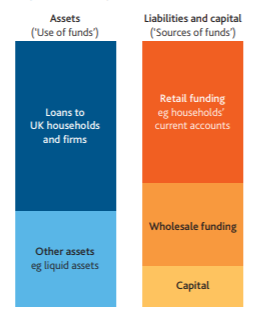
\includegraphics{Figures/simplified_bs.png}
}

\caption{\label{fig:L4_simplified_bs} Simplified bank balance sheet. Source: \href{https://www.bankofengland.co.uk/-/media/boe/files/quarterly-bulletin/2013/bank-capital-and-liquidity.pdf}{Bank of England - Farag (2013)}}

\end{center}
\end{figure}

\end{frame}

%-------------------------------------------------------

%-------------------------------------------------------

\begin{frame}{Composition of assets}

\begin{figure}
\begin{center}

\resizebox{0.70\textwidth}{!}{%
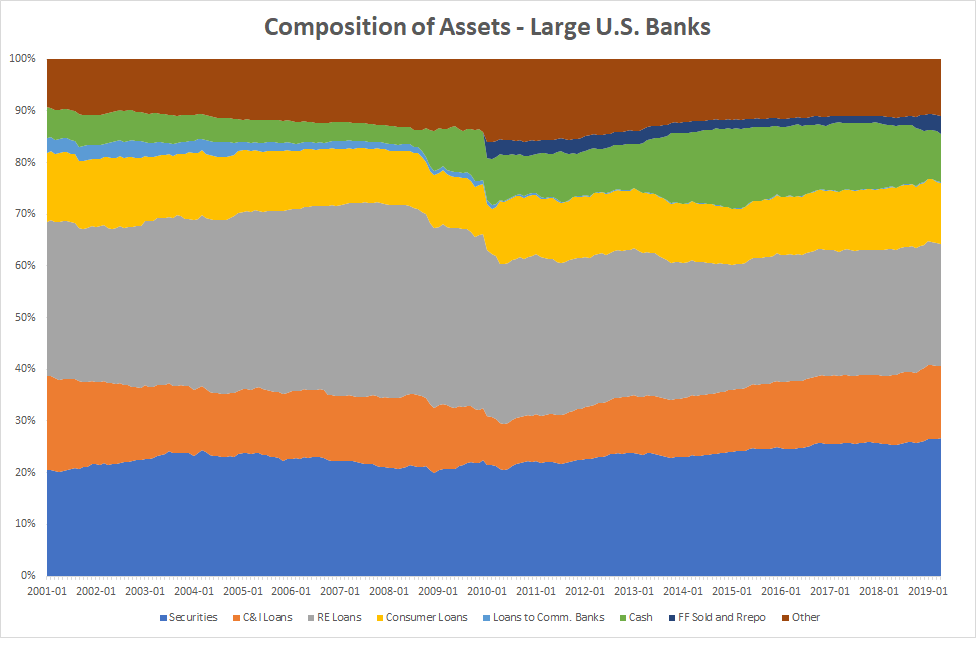
\includegraphics{Figures/Asset_composition_large_banks.png}
}

\caption{\label{fig:L4_Asset_composition_large_banks} Asset composition of large U.S. banks (percent). Source: \href{https://www.federalreserve.gov/releases/h8/current/default.htm}{Federal Reserve table H.8}}

\end{center}
\end{figure}

\end{frame}

%-------------------------------------------------------

%-------------------------------------------------------

\begin{frame}{Composition of liabilities}

\begin{figure}
\begin{center}

\resizebox{0.70\textwidth}{!}{%
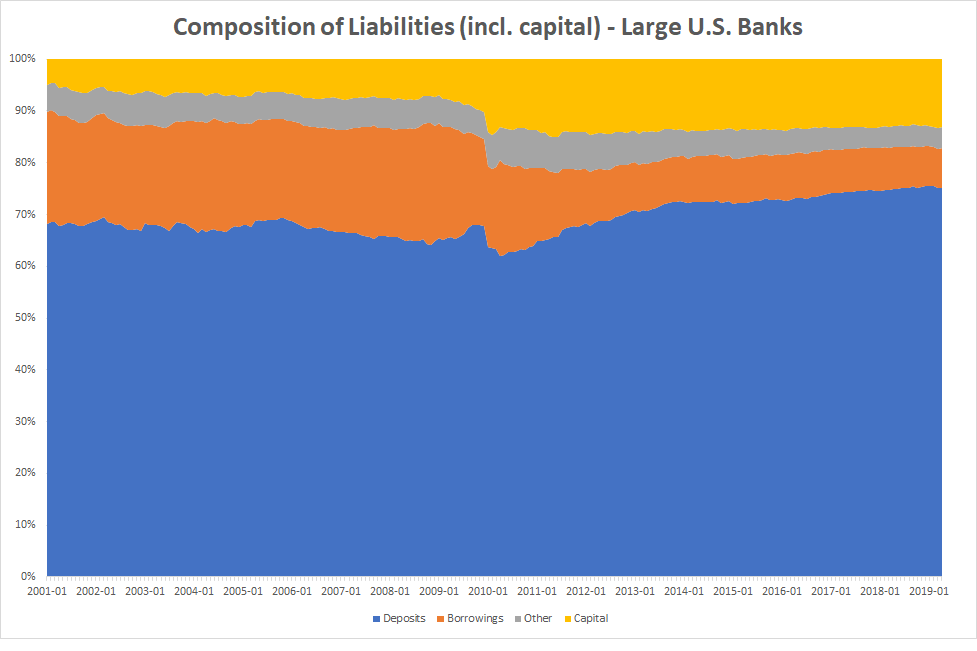
\includegraphics{Figures/Liability_composition_large_banks.png}
}

\caption{\label{fig:L4_Liability_composition_large_banks} Liability (including capital) composition of large U.S. banks (percent). Source: \href{https://www.federalreserve.gov/releases/h8/current/default.htm}{Federal Reserve table H.8}}

\end{center}
\end{figure}

\end{frame}

%-------------------------------------------------------

%-------------------------------------------------------

\begin{frame}{Loans vs. deposits}

\begin{figure}
\begin{center}

\resizebox{0.60\textwidth}{!}{%
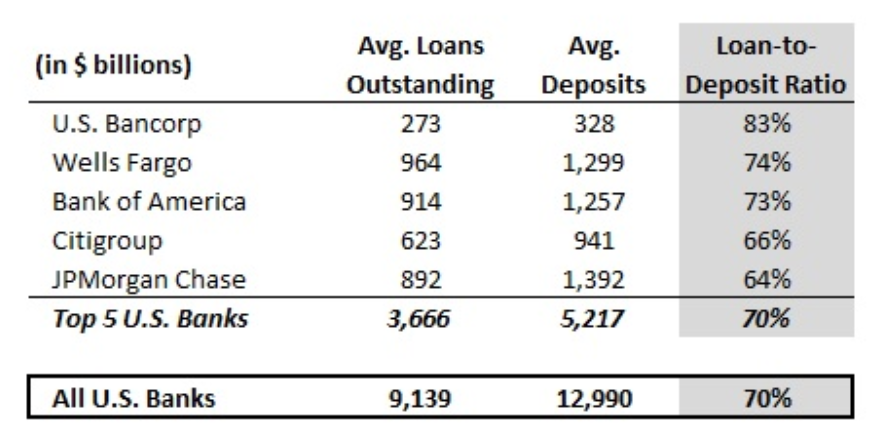
\includegraphics{Figures/2017_loan_to_dep_ratio.png}
}

\caption{\label{fig:L4_2017_loan_to_dep_ratio} Loan to deposit ratios ($2017Q1$). Source: \href{https://www.forbes.com/sites/greatspeculations/2017/06/13/loan-to-deposit-ratios-for-largest-u-s-banks-show-signs-of-recovery-in-q1/\#5d0aa40b12f4}{Forbes (2017)}}

\end{center}
\end{figure}

%Loan-to-deposit ratios (LDRs) across the banking industry have declined steadily since 2010, but some of the largest U.S. banks witnessed a slight uptick in this key metric for Q1 2017 as loan growth outpaced deposit growth. The LDR ratios for the 5 largest banks ranges from around 65\% for JPMorgan Chase and Citigroup to almost 85\% for U.S. Bancorp. The significantly diversified business model for JPMorgan as well as Citigroup (which includes a large custody banking division for both of them) is primarily responsible for their relatively low LDR figures, while U.S. Bancorp’s traditional loans-and-deposits business model explains its higher LDR figure.

%The loan-to-deposit ratio is the ratio of a bank’s total outstanding loans for a period to its total deposit balance over the same period. So an LDR figure of 100\% indicates that a bank lends a dollar to customers for every dollar that it brings in as deposits. But this also means that the bank doesn’t have significant cash on hand for contingencies. A combination of prudence and regulatory requirements suggests that for a traditional bank, the LDR should be around 80-90\%. With a business model that relies heavily on traditional loans-and-deposits services, U.S. Bancorp has an LDR figure that appears to be optimal. As for the other banks, the ratio seems to be inversely proportional to the degree of diversification in the business model – the more diversified the bank in terms of offerings, the lower the LDR figure.

%The Fed’s ongoing rate hike process has improved the interest rate environment – helping deposits grow at a slower rate than loans. This is in contrast to the rapid deposit growth seen over 2011-2016, when low interest rates led to more cash being parked by individuals and institutions with banks. As higher interest rates will provide investors with more lucrative investment options, this will lead to slower growth in deposits. While loans are unlikely to grow at the rapid pace seen over recent years, a strong economic outlook should keep the demand for fresh loans high. This will result in an overall increase in LDR figures over subsequent quarters.

\end{frame}

%-------------------------------------------------------

%-------------------------------------------------------

\begin{frame}{Bank capitalization (inverse of leverage)}

\begin{figure}
\begin{center}

\resizebox{0.90\textwidth}{!}{%
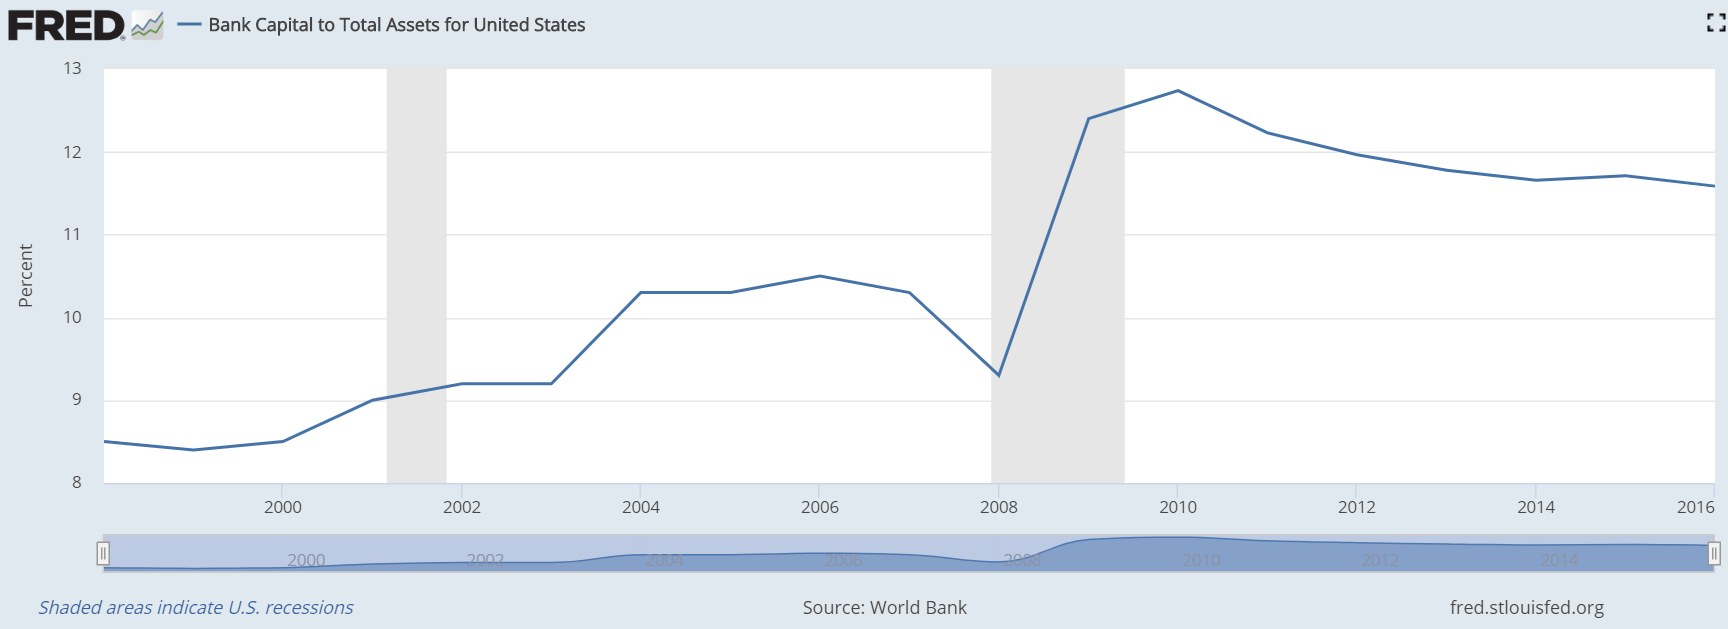
\includegraphics{Figures/US_bank_capital_asset_ratio.png}
}

\caption{\label{fig:L4_US_bank_capital_asset_ratio} Ratio of bank capital and reserves to total assets - variation over time. Source: \href{https://fred.stlouisfed.org/series/DDSI03USA156NWDB}{St Louis Fed. FRED database}}
%Capital and reserves include funds contributed by owners, retained earnings, general and special reserves, provisions, and valuation adjustments. Capital includes tier 1 capital (paid-up shares and common stock), and total regulatory capital, which includes several specified types of subordinated debt instruments which need not be repair if the funds are required to maintain minimum capital levels (these comprise tier 2 and tier 3 capital). Total assets include all nonfinancial and financial assets. 
\end{center}
\end{figure}

\end{frame}

%-------------------------------------------------------

%-------------------------------------------------------

\begin{frame}{Bank balance sheet - solvency after losses}

Suppose a bank initially has a balance sheet of size $\$100$
	\begin{itemize}
	\item	Assets:
		\begin{itemize}
		\item	$\$20$ of risky loans
		\item	$\$70$ of safe loans
		\item	$\$10$ of cash
		\end{itemize}
	\item	Liabilities:
		\begin{itemize}
		\item	$\$x$ of capital
		\item	$\$100 - \$x$ of deposits/wholesale funding/bonds
		\end{itemize}
	\end{itemize}
\vspace{2mm}
Suppose we discover that risky loans were originated under low standards
	\begin{itemize}
	\item	Learn that half are certain to default
	\item	Risky loans revalued to $\$10$
	\end{itemize}
\vspace{2mm}
Importance of initial capital
	\begin{itemize}
	\item	$x=20$ $\Rightarrow$ bank still solvent (capital reduced to $\$10$ but absorbs loss)
	\item	$x=5$ $\Rightarrow$ bank now insolvent (capital is exhausted, assets ($\$90$) $<$ liabilities ($\$95$))
	\end{itemize}

\end{frame}

%-------------------------------------------------------

%-------------------------------------------------------

\begin{frame}{Bank balance sheet - solvency problem}

\begin{figure}
\begin{center}

\resizebox{0.40\textwidth}{!}{%
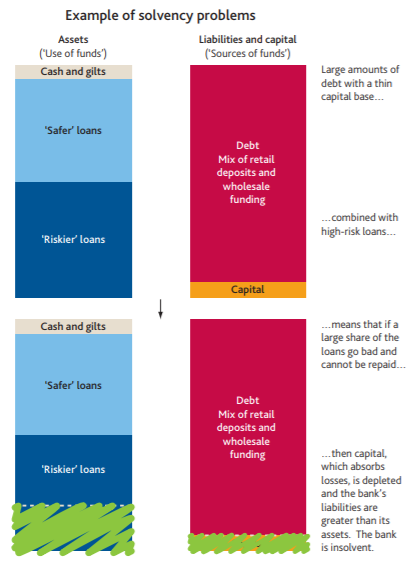
\includegraphics{Figures/bank_bs_solvency_problem.png}
}

\caption{\label{fig:L4_bank_bs_solvency_problem} Simplified bank balance sheet - example of solvency problem. Source: \href{https://www.bankofengland.co.uk/-/media/boe/files/quarterly-bulletin/2013/bank-capital-and-liquidity.pdf}{Bank of England - Farag (2013)}}

\end{center}
\end{figure}

\end{frame}

%-------------------------------------------------------

%-------------------------------------------------------

\begin{frame}{Bank balance sheet - bad loans}

\begin{figure}
\begin{center}

\resizebox{0.90\textwidth}{!}{%
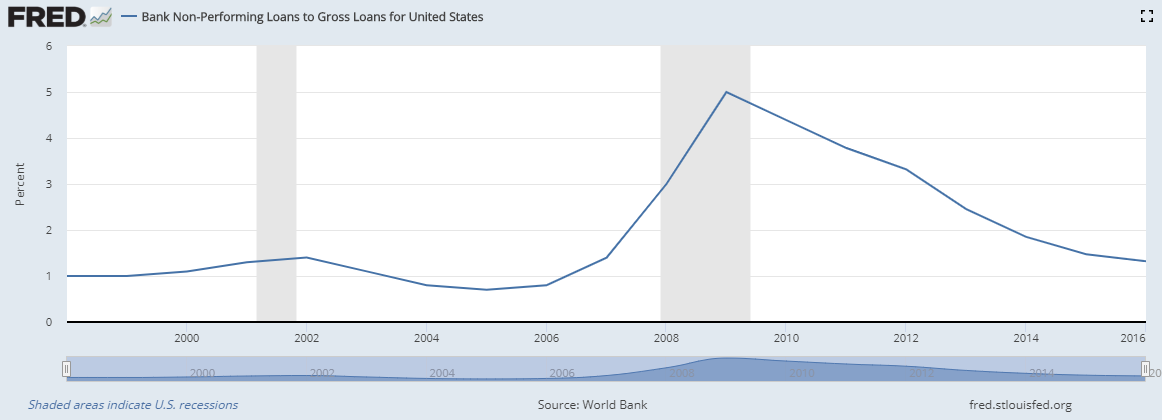
\includegraphics{Figures/NPL_to_total_loans.png}
}

\caption{\label{fig:L4_NPL_to_total_loans} Ratio of defaulting loans (payments of interest and principal past due by 90 days or more) to total gross loans (total value of loan portfolio). Source: \href{https://fred.stlouisfed.org/series/DDSI02USA156NWDB}{St Louis Fed. FRED database}}

\end{center}
\end{figure}

\end{frame}

%-------------------------------------------------------

%-------------------------------------------------------

\begin{frame}{Amplification through leverage}

Why lever up so much?
\vspace{1.5mm}
	\begin{itemize}
	\item	Consider simple example
		\begin{itemize}
		\item	$\$A$ of assets
		\item	$\$x$ of capital (or `equity')
		\item	$\Rightarrow$ `leverage ratio' of $\mathcal{L}=A/x$
		\end{itemize}
	\item	Suppose change in value of assets of $\delta$
		\begin{itemize}
		\item	Shareholders only put up $x$
		\item	Return on their equity is $\frac{\delta}{x}=\frac{A}{x}\frac{\delta}{A}=\mathcal{L}\frac{\delta}{A}$
		\end{itemize}
	\end{itemize}
\vspace{2mm}
Leverage blows up gains (but also amplifies losses)
	\begin{itemize}
	\item	People use the term `capital structure' to refer to the split between `debt' and `equity' in funding
	\item	Leverage typically thought of as total assets / equity
	\end{itemize}
	
\end{frame}

%		\begin{itemize}
%		\item	Bank managers may have short term RoE incentives
%		\item	Regulatory arbitrage arising from poorly designed risk weights
%		\item	Possible anticipation of bailout / `too big to fail'
%		\item	Artificially cheap price of debt (e.g. deposit insurance)
%		\item	Securitization (and regulatory/rating agency treatment of securitized assets)
%		\item	Possible risk shifting (though mainly at low capital levels)
%		\end{itemize}

%-------------------------------------------------------

%-------------------------------------------------------

\begin{frame}{Bank RoA and RoE}

\begin{figure}
\begin{center}

\resizebox{0.90\textwidth}{!}{%
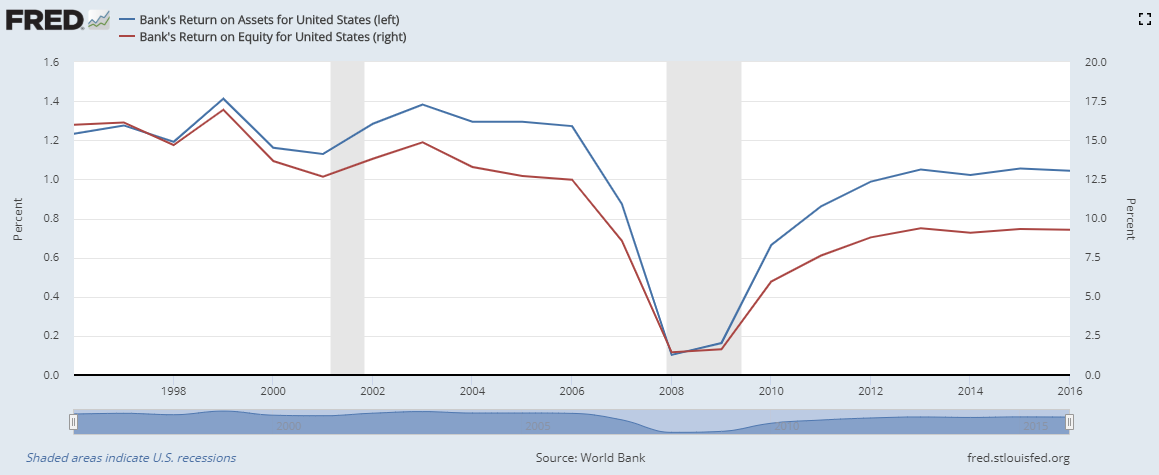
\includegraphics{Figures/roe_and_roa.png}
}

\caption{\label{fig:L4_roe_and_roa} Return on assets (percent, left scale) vs. return on equity (percent, right scale) Source: St Louis Fed. FRED database}

\end{center}
\end{figure}

\end{frame}

%-------------------------------------------------------

%-------------------------------------------------------

\begin{frame}{Models of the importance of capital}

In a perfect world the value of a firm shouldn't depend on capital structure
	\begin{itemize}
	\item	Punchline of the (in)famous \href{https://en.wikipedia.org/wiki/Modigliani\%E2\%80\%93Miller_theorem}{`Modigliani-Miller'} result
	\item	Reallocating payoffs among debt or equity holders shouldn't, \emph{per se}, change value of firm
	\item	Only overall payoff stream from a firm's activity should influence value
	\item	$\Delta$Leverage $\Rightarrow$ $\Delta$Riskiness of debt vs. equity $\Rightarrow$ $\Delta$Prices of debt vs. equity $\Rightarrow$ No $\Delta$Value of firm
	\end{itemize}
\vspace{2mm}
This result holds only in the simplest models and anecdotally there is strong disgareement with it
	\begin{itemize}
	\item	Disagreement may be self-serving (short termist bank managers may want to boost their pay in the short term)
	\item	Strong empirical evidence $\Delta$ equity affects cost of finance	
	\item	Taxes and other (typically information) frictions break the result
	\item	\textbf{Payoffs can depend on capital structure}
	\end{itemize}
	
\end{frame}

%-------------------------------------------------------

%-------------------------------------------------------

\begin{frame}{Models of the importance of capital}

Naive view of credit: If savers have funds to lend, what matters is the entrepreneur's idea and nothing else
	\begin{itemize}
	\item	Either it's a good project or it's not
	\item	How it's funded (bank credit, bonds, equity - some weird type of structured finance) doesn't matter (Modigliani-Miller again)
	\end{itemize}
\vspace{2mm}
Empirical evidence and theoretical work question this
	\begin{itemize}
	\item	\textbf{Financial accelerator} models focused on non-financial firms
		\begin{itemize}
		\item	\textit{Bernanke, Gertler and Gilchrist (1999)}: lenders must pay `auditing cost' to observe a borrower's realized return
		\item	\textit{Kiyotaki and Moore (1997)}: borrowers cannot be forced to repay debts
		\end{itemize}
	\item	Asset price variation induces fluctuations in firms' net worth
	\item	Credit tightens as net worth declines 
	\item	Reduced investment demand can further suppress asset prices
	\item	Vicious circle\ldots
	\end{itemize}

\end{frame}


%-------------------------------------------------------

%-------------------------------------------------------

\begin{frame}{Models of the importance of capital}

\begin{quote}
\ldots when borrowers have little wealth to contribute to project financing, the potential
divergence of interests between the borrower and the suppliers of external funds is
greater, implying increased agency costs; in equilibrium, lenders must be compensated
for higher agency costs by a larger premium [in the lending rate]. To the extent that borrowers' net worth is procyclical (because of the procyclicality of profits and asset prices, for example), the
external finance premium will be countercyclical, enhancing the swings in borrowing
and thus in investment, spending, and production. 
\end{quote}
\begin{center}
- Bernanke, Gertler and Gilchrist (1999)
\end{center}

\end{frame}

%-------------------------------------------------------

%-------------------------------------------------------

\begin{frame}{Models of the importance of bank capital}

\begin{quote}
Traditionally, most economists have regarded the fact that banks hold capital as at best a
macroeconomic irrelevance and at worst a pedagogical inconvenience.
\end{quote}
\begin{center}
- Ben Friedman (1991)
\end{center}

\begin{quote}
The current generation of workhorse models used for monetary policy analysis typically abstract
from imperfections in financial markets. Firms and households can borrow freely at riskless
interest rates. And financial intermediaries, if they are explicitly modeled, are nothing more than
a veil.
\end{quote}
\begin{center}
- Aikman and Paustian (2006)
\end{center}

\end{frame}

%-------------------------------------------------------

%-------------------------------------------------------

\begin{frame}{Models of the importance of bank capital}

Pre-crisis treatment of `banks' in most macro models
	\begin{itemize}
	\item	Simply a conduit for funds to flow from investors to firms
	\item	State of investors and firms might matter but bank health not separately influential
	\item	Not entirely fair: see the (readable) discussion \href{https://www.jstor.org/stable/2138389}{here}
	\end{itemize}
\vspace{2mm}
Yet similar intuitions as for firms apply to banks (banks are also firms!)
	\begin{itemize}
	\item	To the extent that monitoring of firms by banks is costly and unobservable, the bank might want to shirk
	\item	Knowing this, bank investors (e.g. depositors) want bank to have \textit{`skin in the game'}
	\item	By funding their activities partly with their own money (net worth) banks benefit from good performance of loans
	\item	\textbf{Aligns bank's incentives with the interests of bank investors}
	\item	Investors willing to fund bank at a lower rate than otherwise
	\end{itemize}

\end{frame}

%-------------------------------------------------------

%-------------------------------------------------------

\begin{frame}{Models of the importance of bank capital}

Pre-crisis treatment of `banks' in most macro models
	\begin{itemize}
	\item	Simply a conduit for funds to flow from investors to firms
	\item	State of investors and firms might matter but bank health not separately influential
	\item	Not entirely fair: see the (readable) discussion \href{https://www.jstor.org/stable/2138389}{here}
	\end{itemize}
\vspace{2mm}
Yet similar intuitions as for firms apply to banks (banks are also firms!)
	\begin{itemize}
	\item	To the extent that monitoring of firms by banks is costly and unobservable, the bank might want to shirk
	\item	Knowing this, bank investors (e.g. depositors) want bank to have \textit{`skin in the game'}
	\item	By funding their activities partly with their own money (\textcolor{red}{net worth}) banks benefit from good performance of loans
	\item	\textbf{Aligns bank's incentives with the interests of bank investors}
	\item	Investors willing to fund bank \textcolor{red}{at a lower rate than otherwise}
	\end{itemize}

\end{frame}


%-------------------------------------------------------
\section{The Importance of Liquidity}
%-------------------------------------------------------

\begin{frame}

\begin{center}
{\LARGE The Importance of Liquidity}
\end{center}

\end{frame}

%-------------------------------------------------------

%-------------------------------------------------------

\begin{frame}{Liquidity Crisis}

The crisis saw dramatic disruption to, and loss of, liquidity
	\begin{itemize}
	\item	Many ways to define liquidity
	\item	Ability to sell/liquidate asset rapidly at a reasonable price
	\item	Ability to borrow on reasonable terms easily / quickly
	\item	With collateralization, the two definitions are closely related
	\end{itemize}
\vspace{1.5mm}
Liquidity problems interacted with, but to an important degree, are distinct from solvency problems
	\begin{itemize}
	\item	Liquidity: Can I sell assets/borrow quickly at a `fair price'?
	\item	Solvency: Value of assets $>$ liabilities
	\end{itemize}
\vspace{1.5mm}	
Common models of banks' liquidity risk build on \href{https://www.jstor.org/stable/1837095}{Diamond-Dybvig (1983)}
	\begin{itemize}
	\item	Explains how depositors may `run' on `maturity mismatched' banks
	\item	Banks `borrow short and lend long'
	\item	Runs affected banks and shadow banks in the crisis
	\item	Not \href{https://en.wikipedia.org/wiki/Northern_Rock}{(only)} by people \href{https://www.theatlantic.com/business/archive/2016/12/its-a-wonderful-life-banking/511592/}{queuing outside banks} but also in \href{https://www.reuters.com/article/uk-shadow-banking-qa/qa-what-is-shadow-banking-and-why-does-it-matter-idUKTRE81611Q20120207}{debt markets/shadow banking}
	\end{itemize}

\end{frame}

%-------------------------------------------------------

%-------------------------------------------------------

\begin{frame}{Diamond Dybvig (1983)}

Seminal paper: insights into \textit{deep} issues with strikingly sparse model
	\begin{itemize}
	\item	Why maturity transformation by banks might be efficient
	\item	Why this phenomenon also renders them vulnerable to runs
	\item	Why a \textit{solvent} institution might fail, due to a lack of liquidity
	\item	The concept of liquidity - formulated precisely
	\item	Possible policy responses
	\end{itemize}
\vspace{2mm}
The original \href{https://ideas.repec.org/a/ucp/jpolec/v91y1983i3p401-19.html}{\emph{1983 paper}} is readable (one of the great papers)
	\begin{itemize}
	\item	A later summary paper, \href{https://www.richmondfed.org/-/media/richmondfedorg/publications/research/economic_quarterly/2007/spring/pdf/diamond.pdf}{\emph{Diamond (2007)}}, is an easier read
	\end{itemize}

\end{frame}

%-------------------------------------------------------

%-------------------------------------------------------

\begin{frame}{Diamond Dybvig (1983)}
\textbf{Banks borrow\ldots}
		\begin{itemize}
		\item	Liability from perspective of bank
		\item	Asset from perspective of `depositor'
		\item	Also applies to short term borrowing in money markets
		\end{itemize}
\vspace{1mm}		
\textbf{\ldots to fund investments in long(er) term projects}
	\begin{itemize}
	\item	`Illiquid' assets such as loans to build a factory
	\item	Early liquidation may reduce value of asset (loan)
	\end{itemize}
\vspace{4mm}
A principle function of banks is to create liquidity
	\begin{itemize}
	\item	Deposits (withdraw any time at face value) more liquid than assets
	\item	Investors who want liquidity will prefer to hold illiquid assets \emph{indirectly} - through the bank
	\item	This is great - when it works - but there is a nasty sting in the tail!
	\end{itemize}

\end{frame}

%-------------------------------------------------------

%-------------------------------------------------------

\begin{frame}{Diamond Dybvig (1983) - Setup}

\begin{itemize}
\item	One good
\item	Three dates: $t=0,1,2$
\item	Continuum (infinitely many, infinitesimally small) of agents
\item	Each agent endowed with a unit of the good at $t=0$
\item	\emph{Ex ante} the agents are identical (at $t=0$)
\item	But face idiosyncratic shock at $t=1$
	\begin{itemize}
	\item	With (independent) probability $\pi$ they need to consume at period 1
	\item	So with probability $1-\pi$ they need to consume at period 2
	\item	Think of first (`type 1') as impatient and second (`type 2') as `patient'
	\item	Perhaps better to imagine type 1 getting an unexpected cashflow need
	\end{itemize}
\item	As of period $0$ they have utility given by
\[
U = \pi u(C_{1}) + (1-\pi)u(C_{2})
\]
\item	Continuum of agents, independence and LOLN $\Rightarrow$ realized fraction of type 1 at $t=1$ is given by $\pi$
\end{itemize}

\end{frame}

%-------------------------------------------------------

%-------------------------------------------------------

\begin{frame}{Diamond Dybvig (1983) - Alternative `investments'}

Agents can store good from one period to the next without any cost
	\begin{itemize}
	\item	Think of this like sticking money under the mattress
	\end{itemize}
\vspace{2mm}
\textbf{Alternatively} they have access to a constant returns to scale (CRS) technology
	\begin{itemize}
	\item	One unit invested at $t=0 \Rightarrow$ return $R>1$ at $t=2$
	\item	Technology implies an `illiquid asset' in that investment only yields return $s<1$ if it is liquidated at $t=1$
	\item	Think of this as trying to quickly wind up a business or interrupt the building of a factory prematurely
	\end{itemize}
\end{frame}

%-------------------------------------------------------

%-------------------------------------------------------

\begin{frame}{Diamond Dybvig (1983) - Autarky}

Consider an agent (who does not yet know her type) choosing the scale of investment, I, in the CRS technology
\begin{itemize}
\item	Remainder, 1-I, will be stored
\item	There is no trade with the other agent by assumption (autarky) so it is a standalone problem
\end{itemize}

\vspace{2mm}
The concept of \href{https://en.wikipedia.org/wiki/Autarky}{autarky} comes up a lot in economics
\begin{itemize}
\item	Usually as a `bad thing' since trade is good (broadly speaking)
\item	Being `self-sufficient' is good in some contexts - but not when gains from trade are out there!
\item	Autarky is a simple benchmark to show scope for welfare improvement
\item	Often used to represent `punishment' in games (e.g. after a country defaults on debt, models assume it has to face autarky for a certain number of periods before countries/investors trade with them again)
\end{itemize}

\end{frame}

%-------------------------------------------------------

%-------------------------------------------------------

\begin{frame}{Diamond Dybvig (1983) - Autarky}

They look forward in time\ldots
\begin{itemize}
\item	If they turn out to be type 1 they will liquidate (only care about $C_{1}$)
\[
C_{1} = sI + 1- I
\]
\item	If they turn out to be type 2 they will continue project (only care about $C_{2}$)
\[
C_{2} = RI + 1- I
\]	
\item	Anticipating this, they choose $I$ to maximize
\[
\pi_{1}u(sI + 1- I) + (1-\pi_{2})u(RI + 1- I)
\]
\item	The FOC implies
\[
-\frac{1-\pi_{1}}{\pi_{1}} \frac{R-1}{s-1} = \frac{u'(C_{1})}{u'(C_{2})}
\]
\end{itemize}
	
\end{frame}

%-------------------------------------------------------

%-------------------------------------------------------

\begin{frame}{Diamond Dybvig (1983) - Autarky}

We can partially characterize the solution (even without specifying further utility function details)
	\begin{itemize}
	\item	Suppose $I = 0$, then $C_{1}=C_{2}=1$
	\item	Suppose $I = 1$, then $C_{1}=s$ and $C_{2}=R$
	\item	Suppose $I\in(0,1)$ then\ldots
		\begin{itemize}
		\item	$C_{1} = (s-1)I + 1 < 1$ (since $s<1$)
		\item	$C_{2} = (R-1)I + 1 < R - 1 + 1 = R$ (since $R>1$)
		\end{itemize}
	\end{itemize}
\vspace{2mm}
Note that $C_{1}\leq1$ and $C_{2}\leq R$ with at least one strict equality
	\begin{itemize}
	\item	The chosen $I$ is \emph{ex post} inefficient with probability $>0$
	\item	Type $1$: Wish had set $I=0$ as sticking it under the mattress for return of $1$ is better than $s$ from premature liquidation
	\item	Type 2: Wish had set $I=0$ since all savings would have earned $R$, rather than $1$ under the bed
	\item	They do this because they don't want to risk a complete mismatch of payoffs and their liquidity demands
	\end{itemize}
	
\end{frame}

%-------------------------------------------------------

%-------------------------------------------------------

\begin{frame}{Diamond Dybvig (1983) - Opening a financial market}

Is the problem solvable simply by opening a bond market?
	\begin{itemize}
	\item	Price in period 1 of a unit of good in period 2 is given by $p$
	\vspace{1mm}
	\item	Allows type 1 to have $C_{1} = pRI + 1 - I$
		\begin{itemize}
		\item	From selling $RI$ bonds (instead of liquidating long term investment)
		\item	The long term investment allows her to fulfill her commitment
		\end{itemize}
	\vspace{1mm}
	\item	Allows type 2 to have $C_{2} = RI + \frac{1-I}{p}$
		\begin{itemize}
		\item	From buying $\frac{1-I}{p}$ bonds (instead of storing the good for another period)
		\end{itemize}
	\vspace{1mm}
	\item	$C_{1}=pC_{2}$ and thus utility is $\uparrow(\downarrow)$ in $I$ if $pR>1(<1)$
		\begin{itemize}
		\item	Linearity in $I$ implies that an interior solution can only exist if $pR=1$
		\item	Using feasibility $(1-\pi_{1})C_{2} = RI \Rightarrow I = 1-\pi_{1}$
		\end{itemize}
	\vspace{1mm}
	\item	Then $(C_{1},C_{2})=(1,R)$ which is Pareto superior to the autarkic case (where $C_{1}\leq1$ and $C_{2}\leq R$ with at least one - typically both - strict)
	\end{itemize}
\vspace{2mm}
So opening a bond market has improved the situation, but is it `ideal'?

\end{frame}

%-------------------------------------------------------

%-------------------------------------------------------

\begin{frame}{Diamond Dybvig (1983) - Optimal (symmetric) allocation}

Suppose we simply ask what the `planning' optimum would be
\begin{itemize}
\item	We simply maximize $\pi_{1}u(C_{1}) + (1-\pi_{2})u(C_{2})$, subject to
	\begin{itemize}
	\item	Feasibility in period 1: $\pi_{1}C_{1} = 1 - I$
	\item	Feasibility in period 2: $(1-\pi_{1})C_{2} = RI$
	\end{itemize}
\vspace{2mm}	
\item	This is equivalent to choosing $I$ to maximize
\end{itemize}
\[
\pi u\left( \frac{1-I}{\pi_{1}} \right) + (1-\pi_{1}) u \left( \frac{R I}{1-\pi_{1}} \right)
\]
\begin{itemize}
\item This yields the FOC that optimal allocation $(C^{\ast}_{1},C^{\ast}_{2})$ must satisfy
\end{itemize}
\[
-u'(C^{\ast}_{1}) + Ru'(C^{\ast}_{2}) = 0
\]
\textbf{\href{https://en.wikipedia.org/wiki/Generic_property}{Generically} the (bond) market allocation won't satisfy this condition}
	\begin{itemize}
	\item	Need fluke $u(\cdot)$ for it to hold with $(C_{1},C_{2})=(1,R)$ (implying $I=1-\pi_{1}$)
	\end{itemize}

\end{frame}

%-------------------------------------------------------

%-------------------------------------------------------

\begin{frame}{Diamond Dybvig (1983) - Banking equilibria}

It turns out that the presence of banks can implement the optimum, as \textbf{an} equilibrium
\begin{itemize}
\item	Suppose we have a fractional reserve system
	\begin{itemize}
	\item	Not all deposits are backed by short term assets
	\end{itemize}
\item	The bank\ldots
	\begin{itemize}
	\item	Collects agents' endowments in time 0 (deposits)
	\item	Offers the depositors the right to withdraw at any time
	\item	Invests a fraction in the long-term project
	\item	Proposes a deposit contract that allocates $(C_{1}^{\ast},C_{2}^{\ast})$ in periods 1 and 2, respectively, given a unit deposit in period 0
	\end{itemize}
\end{itemize}

\end{frame}

%-------------------------------------------------------

%-------------------------------------------------------

\begin{frame}{Diamond Dybvig (1983) - Banking equilibria}

Good equilibrium
	\begin{itemize}
	\item	Suppose type 2 agent (whose beliefs matter) believes bank will satisfy its obligations in period 2
	\item	The FOC from the planning problem $\Rightarrow$ $C_{1}^{\ast}< C_{2}^{\ast}$ so sticking with the contract is preferable to withdrawing and storing
	\item	All type 1 agents will withdraw - so the bank must have $\pi_{1}C_{1}^{\ast}$ on hand
	\item	So the bank must invest only $1-\pi_{1}C_{1}^{\ast}$ in project at $t=0$
	\item	Then the bank is solvent in this equilibrium with probability $1$
	\end{itemize}

\end{frame}

%-------------------------------------------------------

%-------------------------------------------------------

\begin{frame}{Diamond Dybvig (1983) - Banking equilibria}

Bad equilibrium (bank run)
	\begin{itemize}
	\item	Suppose bank adopts the approach above but\ldots
	\item	Suppose a type 2 agent believes all other type 2 will withdraw at $t=1$
	\item	Then bank will need to liquidate all its assets at $t=1$ yielding total value $\pi_{1} C_{1}^{\ast} + (1-\pi_{1}C_{1}^{\ast})s < 1 < C_{1}^{\ast}$ ($C_{1}^{\ast}$ is the value of its liabilities)
	\item	$\Rightarrow$ insolvent and nothing will remain to pay out in period 2
	\item	So, given these beliefs, optimal for (any and all) type 2 agents to withdraw in $t=1$
	\item	Behavior confirms the belief that induced it $\Rightarrow$ an equilibrium
	\end{itemize}
\vspace{2mm}
Deposit insurance or bailing banks out can prevent this, but\ldots
	\begin{itemize}
	\item	Dulls depositors' incentive to monitor banks and - unless properly priced - subsidizes risky investments
	\item	Huge problems with moral hazard if banks anticipate bailout
	\end{itemize}

\end{frame}

%-------------------------------------------------------

%-------------------------------------------------------

\begin{frame}{Other models of liquidity crises and runs}

There are various ways of modeling runs and liquidity crunches
\begin{itemize}
\item	Other frameworks relevant to the recent crisis are those that emphasize fire-sales
\item	There can be important feedbacks from fire-sales, depressing asset prices, to weakening of banks, requiring further sales and difficulty in obtaining funding with collateralized borrowing\ldots
\end{itemize}

\end{frame}

%-------------------------------------------------------

%-------------------------------------------------------

\begin{frame}{Vicious circles in funding and asset prices}

\begin{figure}
\begin{center}

\resizebox{0.70\textwidth}{!}{%
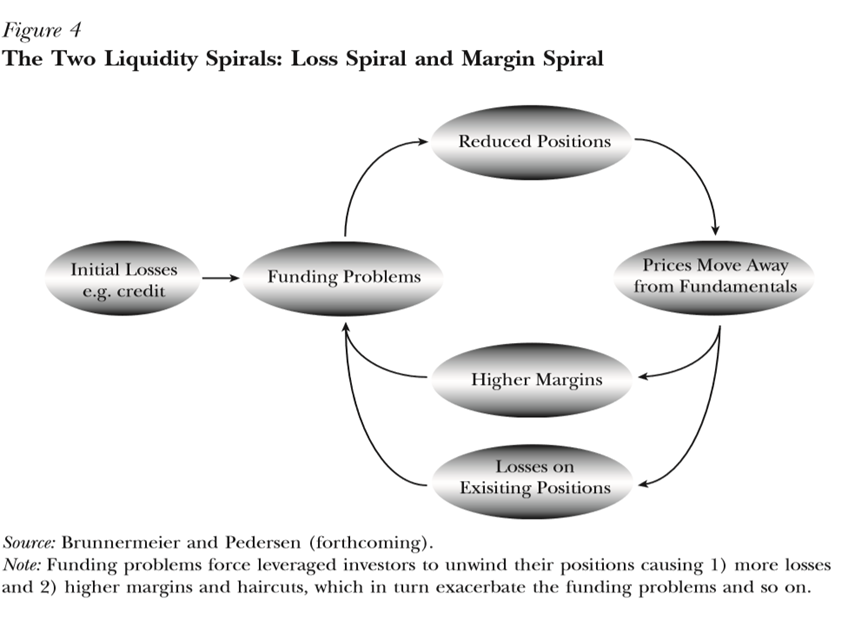
\includegraphics{Figures/liquidity_spiral.png}
}

\caption{\label{fig:L4_liquidity_spiral} Liquidity spirals feeding back into fire sales and asset price declines, feeding back into liquidity spirals\ldots. Source: \href{https://www.princeton.edu/~markus/research/papers/liquidity_credit_crunch.pdf}{Brunnermeier (2009); Bloomberg}}

\end{center}
\end{figure}

\end{frame}



%-------------------------------------------------------
\section{Pre-crisis Vulnerabilities}
%-------------------------------------------------------

\begin{frame}

\begin{center}
{\LARGE Pre-crisis Vulnerabilities}
\end{center}

\end{frame}

%-------------------------------------------------------

%-------------------------------------------------------

\begin{frame}{Pre-crisis vulnerabilities}

\begin{figure}
\begin{center}

\resizebox{0.65\textwidth}{!}{%
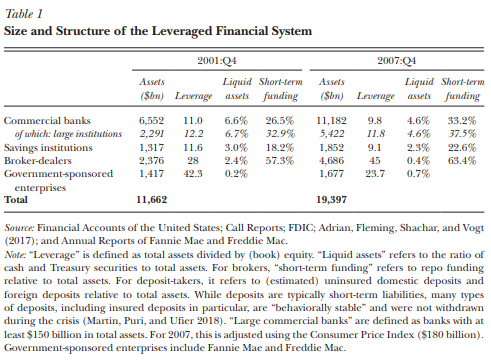
\includegraphics{Figures/aikman_et_al_banks_bs_pre_crisis.png}
}

\caption{\label{fig:L4_aikman_et_al_banks_bs_pre_crisis} Buildup of vulnerabilities from $2001$ to $2007$ - solvency, liquidity and funding. Source: \href{https://pubs.aeaweb.org/doi/pdfplus/10.1257/jep.33.1.107}{Aikman \emph{et al} (2019)}}

\end{center}
\end{figure}

%The most extreme vulnerabilities developed for the parts of the financial
%system that did not take traditional deposits. Consider, for instance, the changes
%for broker-dealers, a category that includes specialised investment banks and the
%investment banking subsidiaries of larger banking groups. The assets of these entities increased from 28 to 45 times their equity between 2001 and 2007, meaning that
%a roughly 2 percent decline in the value of broker-dealers’ assets would have been
%sufficient to wipe out all of their equity. In addition, these firms were traditionally
%highly reliant on short-term wholesale funding (Rosengren 2014), and became even
%more so during this period.
%Much of this short-term funding took the form of repurchase agreements, or
%“repos.” Repos are a form of borrowing in which the broker-dealer sells securities
%that it holds, receives the value of those securities in cash, and a few days later repurchases the securities at a predetermined price that includes an additional interest
%payment. The repo liabilities of broker-dealers increased from $1.4 trillion in 2001
%to $3.0 trillion in 2007.1
% Moreover, an increasing fraction of repos were backed by
%low-quality securities. 

\end{frame}

%-------------------------------------------------------

%-------------------------------------------------------

\begin{frame}{Off balance sheet exposures}

\begin{figure}
\begin{center}

\resizebox{0.70\textwidth}{!}{%
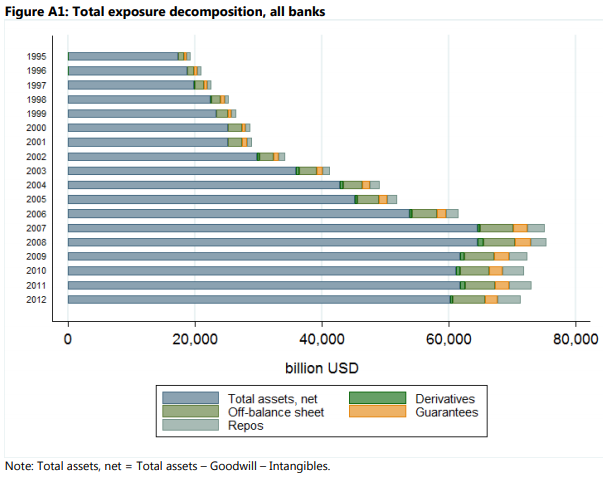
\includegraphics{Figures/total_exposure_incl_derivs_off_bs.png}
}

\caption{\label{fig:L4_total_exposure_incl_derivs_off_bs} Adjusting total exposure for derivatives and off-balance-sheet positions. Source: \href{https://www.bis.org/publ/work471.pdf}{Brei and Gambacorta (2014)}}

\end{center}
\end{figure}

\end{frame}

%-------------------------------------------------------

%-------------------------------------------------------

\begin{frame}{Risk weight `optimization' (regulatory arbitrage)}

\begin{figure}
\begin{center}

\resizebox{0.70\textwidth}{!}{%
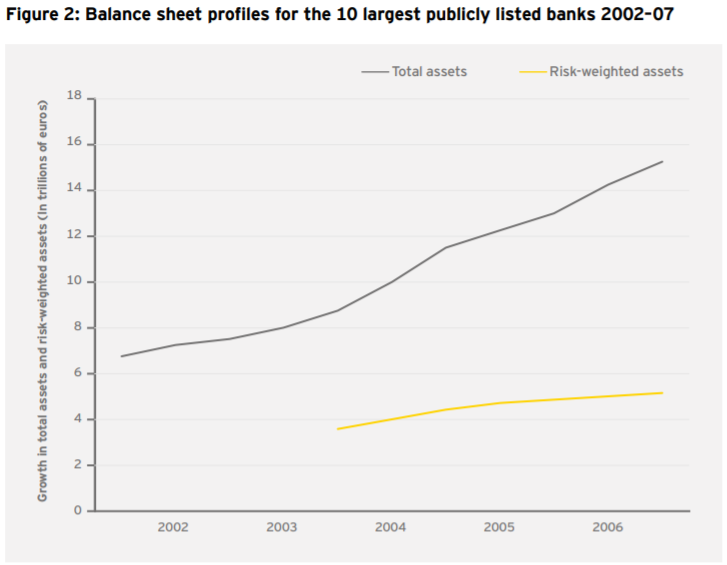
\includegraphics{Figures/ey_ta_rwa_note.png}
}

\caption{\label{fig:L4_ey_ta_rwa_note} Approximate constancy of capital ratios with respect to risk weighted assets vs. buildup of leverage. Source: EY, Avgouleas and Cullen (2015); IMF}

\end{center}
\end{figure}

%While asset levels increased markedly in the years leading up to the GFC, reported leverage
%levels at large commercial banks were remarkably constant. This would normally suggest
%that while banks expanded asset levels aggressively they maintained capital levels and
%preserved stable leverage ratios [Kalemli-Ozcan et al. (2012)]. However, official data
%does not provide the full picture. Leverage increases were caused by poorly calibrated
%internal financial models [Simkovic (2009)], the poor performance of credit rating agencies
%[Johnston (2011)], and fraud [Valukas (2010)].
%Moreover, there is strong evidence that reported leverage levels at both commercial and
%investment banks were manipulated, or were inaccurate, due to exploitation of prevalent
%rules on bank capital by bank management. For example, banks switched away from loans
%into structured financial products, which benefitted from higher capital relief. The increased
%role of complex securitized credit and marketable securities provided additional avenues
%to augment bank capital structures [Stein (2010)]. Under the Basel Accords, the lower risk
%weights that securitized products attracted meant that banks did not have to hold the same
%levels of capital against those assets, as it would be the case if the underlying products were
%not securitized. Basel II, in particular, made few significant changes to regulatory capital
%requirements in relation to conduits, leading to a reduction in overall capital requirements.
%Much risk-weighted optimization (RWO) was achieved through employment of securitization
%models, as it was assumed that by diversifying and spreading risk throughout the financial
%system through securitization, the financial system would be more stable and more resilient
%to shocks [Blair (2013)]. These conduits raised funds by selling short-term asset-backed
%commercial paper, with the assets concerned usually comprising mortgage pools and
%secured loans. Because these conduits funded themselves with short-term debt, any loss of
%confidence or liquidity pressures due to a reduction in buyers of commercial paper would
%quickly destroy their viability, indirectly exposing the sponsor bank to funding liquidity risk.
%The dual advent of risk-weighted capital requirements and financial innovation for funding
%has hereto enabled banks to engage in RWO for the best part of the past two decades.
%Indeed, research confirms that RWO has not abated since the GFC [Blundell-Wignall and
%Atkinson (2012)]. This has resulted in several large European banks operating with relatively
%low levels of common equity, despite being “well-capitalized” in terms of tier-1 risk-based
%capital (Figure 3).

\end{frame}

%-------------------------------------------------------

%-------------------------------------------------------

\begin{frame}{Enormous expansion of leverage}

Banks (and other financial intermediaries) were highly levered
	\begin{itemize}
	\item	Especially if one looks at raw (not risk-weighted) assets
	\end{itemize}
\vspace{2mm}
Plentiful supply of funds
	\begin{itemize}
	\item	Partly a search for yield
	\item	Developing countries - esp. oil producers - looking to invest using their `savings glut'
	\end{itemize}
\vspace{2mm}
Misspricing and unawareness of risks of innovative, opaque and poorly understood asset classes which often collateralized debt
	\begin{itemize}
	\item	Regulators, risk weights
	\item	Ratings agencies
	\item	Market participants
	\end{itemize}
\vspace{2mm}
Also reflected highly profitable (for a time) `originate and distribute' model\ldots
	
\end{frame}

%-------------------------------------------------------

%-------------------------------------------------------

\begin{frame}{Originate and distribute}

Traditionally banks originated loans and then held them on their balance sheet
\begin{itemize}
\item	Incentive to keep monitoring them and make good loans to begin with
\end{itemize}
\vspace{2mm}
Arguably the `market' can improve on this
\begin{itemize}
\item	Banks may not be the natural holders of the various types of risks involved - even if they are good at originating loans (vetting borrowers etc.)
\end{itemize}
\vspace{2mm}
Securitization (supposedly) allowed banks to `distribute' the loans
	\begin{itemize}
	\item	Shift a pool of loans to special purpose vehicles (SPVs)
	\item 	SPVs issue asset backed commercial paper (or MBS if they were pools of mortgages)
	\item	This CP allows the loans to be funded `off balance sheet' of the bank (with perhaps an explicit or implicit back-up line of credit)
	\end{itemize}

\end{frame}

%-------------------------------------------------------

%-------------------------------------------------------

\begin{frame}{Originate and distribute}

Why might OaD promote lending? Optimistic answer\ldots
	\begin{itemize}
	\item	Improves liquidity (lowers borrowing rates)
		\begin{itemize}
		\item	Might allow banks to de-risk or raise funds more quickly under stress
		\item	See Loutskina (2011) and Bidder \emph{et al} (2019)
		\end{itemize}
	\vspace{2mm}
	\item	Reduces risk through diversification and a broader investor base
		\begin{itemize}
		\item	Tranching of asset pools allowed creation of derivative assets with different risk classes
		\item	Some investors (e.g. money market funds) can only invest in AAA
		\item	AAA can be synthesized by `last loss' or `super senior' tranche of CDOs
		\item	Interesting literature on the shortage of public provision of `riskless assets' (see Krishnamurthy and Caballero's work) inducing private sector to fill the void
		\end{itemize}
	\end{itemize}
\vspace{2mm}
\textbf{But banks were buying a lot of the derivatives - so risk was staying within the system!}
\end{frame}


%-------------------------------------------------------

%-------------------------------------------------------

\begin{frame}{Originate and distribute}

Why might OaD promote lending? More cynical (realistic) answer\ldots
	\begin{itemize}
	\item	Preferential regulatory treatment of off-balance sheet item
		\begin{itemize}
		\item	Less capital required despite same risk (possibly endogenously worse)
		\item	Capital held against loans $>$ capital held against backup lines of credit
		\end{itemize}
	\vspace{0.5mm}
	\item	Private securitization (esp. of subprime mortgages and ABCP) helped artificially stimulate credit  - \href{https://academic.oup.com/qje/article-abstract/125/1/307/1880343?redirectedFrom=fulltext}{Keys \emph{et al} (2010)}.
		\begin{itemize}
		\item	Eventually seemed to induce declines in lending standards
		\item	Low-documentation, NINJA and ARMs became prevalent
		\item	Senior Loan Office Surveys also indicated excessive loosening
		\item	Homeowners encouraged to extract equity (aggregate LTV $\approx$ flat despite price rises)	
		\end{itemize}
	\end{itemize}

\vspace{2mm}
Research by \href{https://academic.oup.com/qje/article-abstract/128/4/1687/1849337}{Mian and Sufi (2013)} $\Rightarrow$ debt was an important transmission mechanism to the broader economy
		\begin{itemize}
		\item	Fine until \textbf{aggregate} U.S. house prices slowed/turned
		\item	Overleveraged households (or states where they were prevalent) suffered the most when the cycle turned
		\end{itemize}
	
\end{frame}

%-------------------------------------------------------

%-------------------------------------------------------

\begin{frame}{Mortgage debt and house price growth (and collapse)}

\begin{figure}
\begin{center}

\resizebox{0.60\textwidth}{!}{%
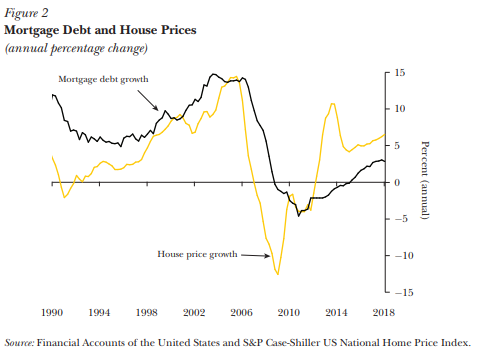
\includegraphics{Figures/aikman_et_al_house_prices_mortage.png}
}

\caption{\label{fig:L4_aikman_et_al_house_prices_mortage} Rapid run-up (and then crash) in mortgage debt growth and U.S. house prices. Source: \href{https://pubs.aeaweb.org/doi/pdfplus/10.1257/jep.33.1.107}{Aikman \emph{et al} (2019)}}

\end{center}
\end{figure}

%Mortgage debt doubled in the six years before the
%crisis, and by 2007 reached 72 percent of GDP. Two aspects of this debt build-up are
%noteworthy and will inform our later macroprudential analysis.
%First, the increase in mortgage debt was accompanied by a house price boom,
%shown in Figure 2. House prices rose by two-thirds in the five years to their peak in
%early 2006 (according to the S&P Case-Shiller US National Home Price Index), and
%ongoing rapid house price appreciation was embedded in expectations (Gennaioli
%and Shleifer 2018). The aggregate loan-to-value ratio on the stock of US housing
%remained broadly flat during this period, meaning that for each 1 percent increase
%in house values, homeowners also increased their mortgage debt by around
%1 percent. In part, this reflected new homeowners taking out larger mortgages in
%order to purchase more expensive homes. But in addition, existing homeowners
%also extracted housing equity by taking out additional debt. Mian and Sufi (2011)
%estimate that existing homeowners borrowed $0.25 on average for every $1 increase
%in home-equity value during the housing boom, enough to account for over half of
%the increase in debt for homeowners between 2002 and 2006.
%Second, there were clear signs in the years before the financial crisis that lending
%standards were being loosened and borrower quality was deteriorating. The Federal
%Reserve Board’s Senior Loan Officer Opinion Survey on Bank Lending Practices
%reported easing standards between 2004Q1 and 2006Q3. The expansion of credit to
%the most risky borrowers was particularly pronounced. For example, according to the
%Federal Reserve’s Survey of Consumer Finances, the share of the stock of mortgagors
%with debt of over four times their income more than doubled between 2001 and 2007
%from 6 percent to 13 percent. The number of new subprime mortgages nearly doubled
%between 2003 and 2005, 80 percent of which were made with short-term “teaser” interest
%rates (in this journal, Mayer, Pence, and Sherlund 2009). “Near-prime” mortgages also
%increased rapidly. The private-label securitization market, in which these mortgages
%were bundled into tranched financial securities and resold, was an important driver of
%these frothy credit supply conditions (Keys, Mukherjee, Seru, and Vig 2010).

\end{frame}

%-------------------------------------------------------

%-------------------------------------------------------

\begin{frame}{Commercial paper buildup - especially asset-backed}

\begin{figure}
\begin{center}

\resizebox{0.70\textwidth}{!}{%
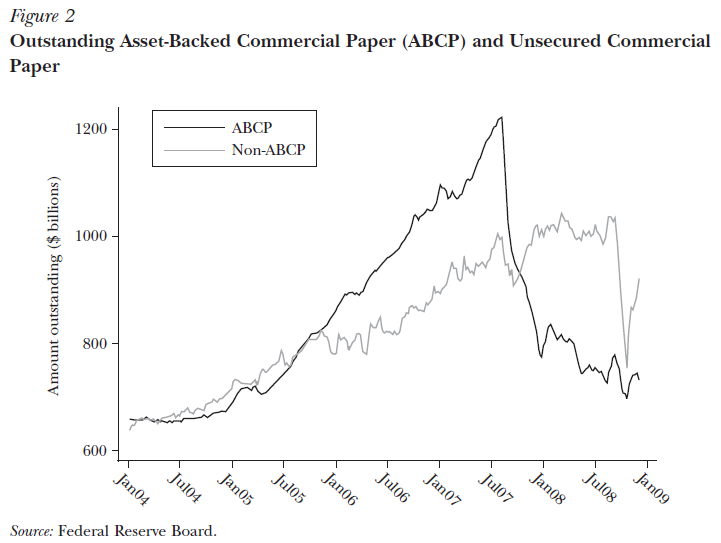
\includegraphics{Figures/ABCP_cliff.png}
}

\caption{Buildup and then collapse in ABCP (eventually followed by non-asset backed paper). Source: \href{https://www.princeton.edu/~markus/research/papers/liquidity_credit_crunch.pdf}{Brunnermeier (2009); Bloomberg}}

\end{center}
\end{figure}

\end{frame}

%-------------------------------------------------------

%-------------------------------------------------------

\begin{frame}{Additional vulnerabilities}

Increased opacity of assets and counterparty interlinkages
	\begin{itemize}
	\item	Companies (e.g. AIG) that weren't on the radar, become enormously interlinked through insuring CDOs etc.
	\item	Fine while agents are looking for `informationally insenstive' assets, but disastrous when people were trying to reasses
	\item	In the absence of liquid markets the assets are very difficult to price / learn about - so arbitrary beliefs can be held\ldots
	\end{itemize}
\vspace{2mm}
Shortened maturity of debt (recall Diamond-Dybvig!)
	\begin{itemize}
	\item	Large banks used short maturity repo to roll massive amounts of debt
	\item	No `deposit insurance' for repo!
	\item	$3$-month repo fairly constant but overnight increased substantially
	\item	Tapping money market funds on basis of (implausible) AAA ratings
	\item	Off-balance sheet lines of credit for SPV were a \textit{time bomb}
	\end{itemize}

\end{frame}

%-------------------------------------------------------

%-------------------------------------------------------

\begin{frame}{Additional vulnerabilities}

Repo (or a `repurchase agreement')
	\begin{itemize}
	\item	A form of collateralized borrowing
	\item	Borrower sells an asset to the lender at a `haircut'
	\item	Promises to buy at back at maturity plus interest
	\item	Simple summaries \href{https://www.investopedia.com/terms/r/repurchaseagreement.asp}{here}, \href{https://en.wikipedia.org/wiki/Repurchase_agreement}{here} and \href{https://www.icmagroup.org/Regulatory-Policy-and-Market-Practice/repo-and-collateral-markets/icma-ercc-publications/frequently-asked-questions-on-repo/3-what-is-the-role-of-repo-in-the-financial-markets/}{here} (see also the Gorton-Metrick `run on repo' paper in the readings - early sections)
	\end{itemize}

\end{frame}

%-------------------------------------------------------

%-------------------------------------------------------

\begin{frame}{Additional vulnerabilities}

\begin{figure}
\begin{center}

\resizebox{0.50\textwidth}{!}{%
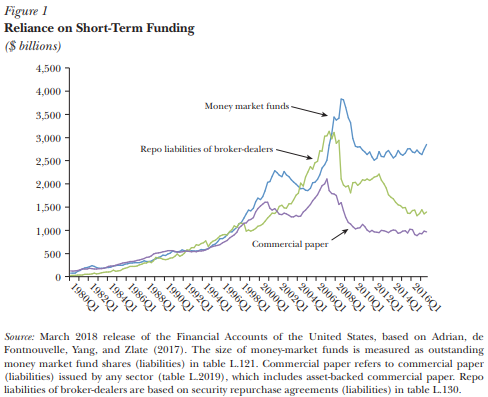
\includegraphics{Figures/aikman_et_al_short_term_funding.png}
}

\caption{\label{fig:L4_aikman_et_al_short_term_funding} Buildup of vulnerabilities from $2001$ to $2007$ - increased use of repo and other short term funding and the absorption of this debt by money market funds. Source: \href{https://pubs.aeaweb.org/doi/pdfplus/10.1257/jep.33.1.107}{Aikman \emph{et al} (2019)}}

\end{center}
\end{figure}

%Figure 1 shows the rise in repo funding, along with commercial paper, another
%form of funding that experienced rapid growth over this period. Traditional commercial paper is short-term debt issued by companies to fund operations. However, by
%the end of 2006, 60 percent of outstanding commercial paper consisted of so-called
%“asset-backed commercial paper” that had been issued to fund the purchase of specific
%securities such as credit card receivables, auto loans, or mortgage-backed securities.
%The growth in repos and commercial paper coincided with an increase in
%the size of money market mutual funds, which purchased much of the repos and
%commercial paper issued. Regulators allowed money market mutual funds to invest
%in assets with a weighted average maturity of up to 90 days, but these funds offered
%investors the ability to withdraw their money at a day’s notice. Moreover, money
%market mutual funds did not have any capital that would shield these short-term
%investors from losses. In a crisis, investors in money market mutual funds who withdrew their funds first were certain to be fully paid, while later claims might not be
%fully paid, providing incentives to “run” on the fund.
%In summary, nonbanks became an increasingly important source of credit for
%the real economy in the years preceding the crisis: between 2001 and 2007, nonbank
%financials accounted for over 70 percent of the total growth in home mortgage
%credit (according to the Financial Accounts of the United States). This growth was
%accompanied by an increased reliance on debt financing of the nonbank system.
%Short-term borrowing became more important, with the belief that it could be rolled over continually

\end{frame}

%-------------------------------------------------------

%-------------------------------------------------------

\begin{frame}{Still dancing\ldots}

\begin{quote}
When the music stops, in terms of liquidity, things will be complicated. But as long as the music is playing, you’ve got to get up and dance. We’re still dancing.
\end{quote}
\begin{center}
- Chuck Prince, Citi CEO, July 10, 2007
\end{center}

\end{frame}

%-------------------------------------------------------
\section{The Crisis}
%-------------------------------------------------------

\begin{frame}

\begin{center}
{\LARGE The Crisis}
\end{center}

\end{frame}

%-------------------------------------------------------

%-------------------------------------------------------

\begin{frame}{Housing market and mortgage debt}

\begin{figure}
\begin{center}

\resizebox{0.70\textwidth}{!}{%
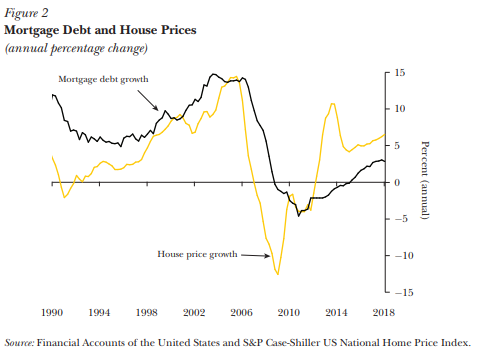
\includegraphics{Figures/aikman_et_al_house_prices_mortage.png}
}

\caption{House prices and mortgage debt. Source: \href{https://pubs.aeaweb.org/doi/pdfplus/10.1257/jep.33.1.107}{Aikman \emph{et al} (2019)}}

\end{center}
\end{figure}

\end{frame}

%-------------------------------------------------------

%-------------------------------------------------------

\begin{frame}{Rapid deterioration of MBS market}

\begin{figure}
\begin{center}

\resizebox{0.38\textwidth}{!}{%
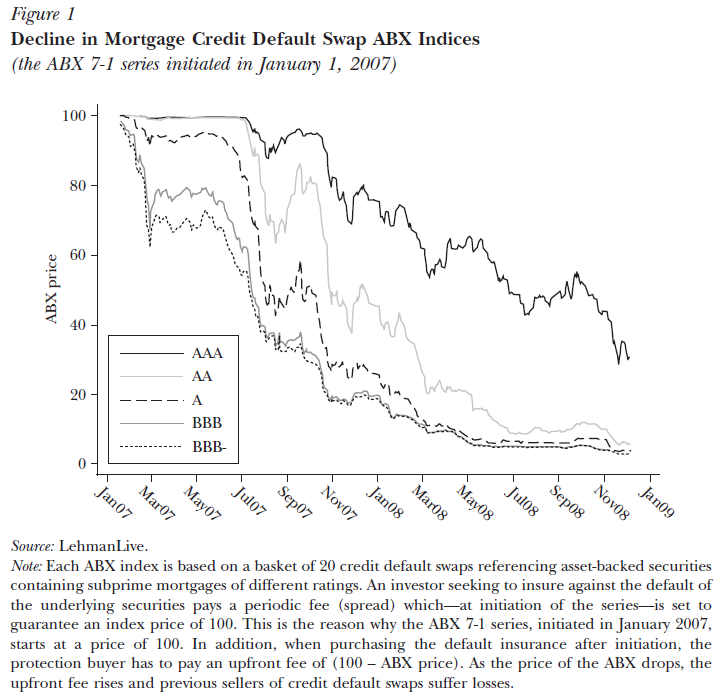
\includegraphics{Figures/ABX_indices.png}
}

\caption{\label{fig:L4_ABX_indices}  Source: \href{https://www.princeton.edu/~markus/research/papers/liquidity_credit_crunch.pdf}{Brunnermeier (2009); Bloomberg}}

\end{center}
\end{figure}

\begin{itemize}
\item	Sudden deterioration in sentiment in MBS markets
\item	Reflects higher (perceived) probabilities of systematic defaults in pools
\item	House-price slowdown and some funds needing parent support
\end{itemize}

\end{frame}

%-------------------------------------------------------

%-------------------------------------------------------

\begin{frame}{Shutdown of asset backed commercial paper markets}

\begin{figure}
\begin{center}

\resizebox{0.55\textwidth}{!}{%
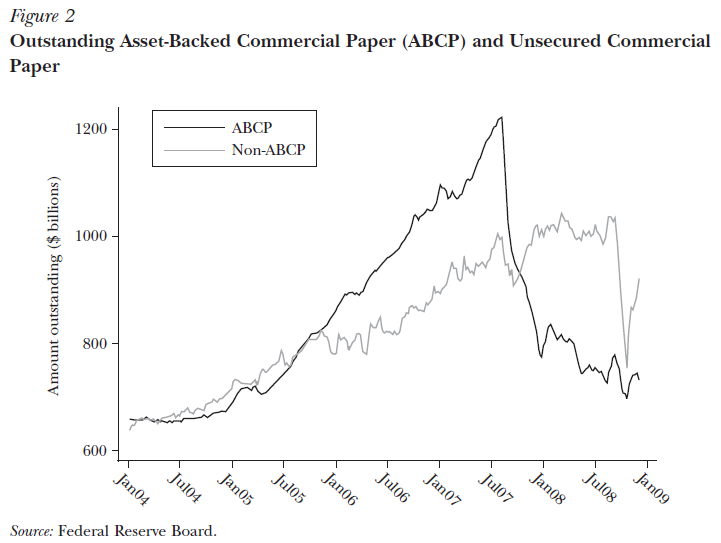
\includegraphics{Figures/ABCP_cliff.png}
}

\caption{\label{fig:L4_ABCP_cliff} Collapse in ABCP (eventually followed by non-asset backed paper). Source: \href{https://www.princeton.edu/~markus/research/papers/liquidity_credit_crunch.pdf}{Brunnermeier (2009); Bloomberg}}

\end{center}
\end{figure}

\begin{itemize}
\item	Note the initial impact is in the \emph{asset backed} segment
\end{itemize}

\end{frame}

%-------------------------------------------------------

%-------------------------------------------------------

\begin{frame}{Fear in the interbank markets}

\begin{figure}
\begin{center}

\resizebox{0.60\textwidth}{!}{%
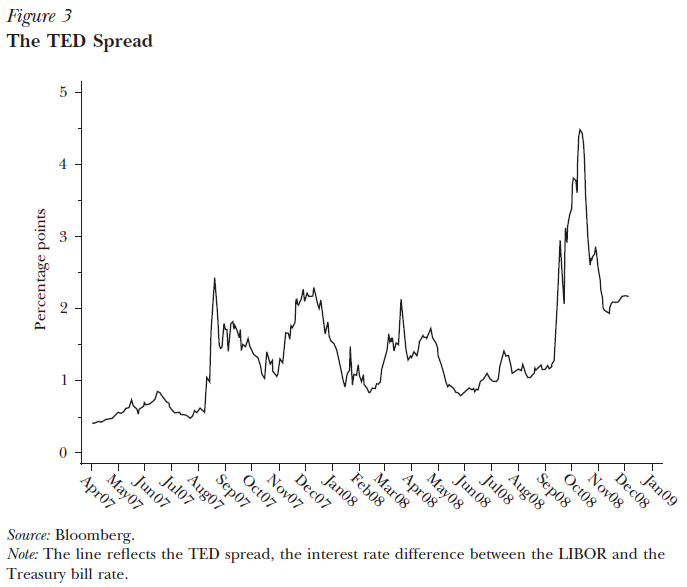
\includegraphics{Figures/ted_spread.png}
}

\caption{\label{fig:L4_ted_spread} Ted spread: 3-Mo LIBOR - 3-Mo T-Bill as a measure of interbank funding difficulties}

\end{center}
\end{figure}

\end{frame}

%-------------------------------------------------------

%-------------------------------------------------------

\begin{frame}{Fear in the interbank markets}

\begin{figure}
\begin{center}

\resizebox{0.80\textwidth}{!}{%
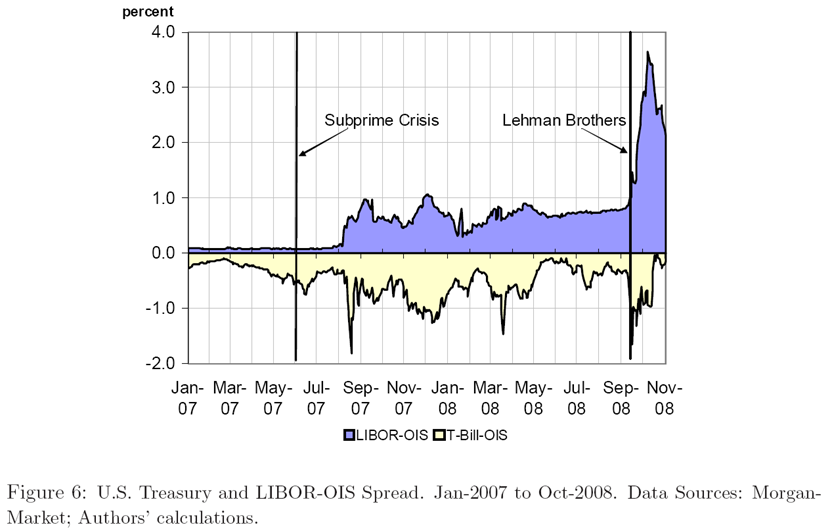
\includegraphics{Figures/caballero_et_al_ted_spread.png}
}

\caption{\label{fig:L4_ted_spread_and_liquidity} Decomposing Ted-spread into `risk' and `liquidity'. Source: Caballero, Fahri and Gourinchas (2008) - also see \href{https://www.investopedia.com/articles/active-trading/061114/what-ois-libor-spread-and-what-it.asp}{here}}

\end{center}
\end{figure}

%Most likely, the strong U.S. capital inflows of the last few years contributed to the significant weakening of U.S. credit markets. The eventual recognition of their degraded performance was one of the triggers of the current crisis. However, this weakening is in itself
%part of the endogenous response of U.S. financial markets to world financial conditions. In
%effect, U.S. assets became stretched by trying to accommodate the world’s excess demand
%for assets. Therein lies the structural problem. This chronic excess demand for assets derives from financial underdevelopment in emerging markets and most commodity producing
%economies, rather than from macroeconomic imbalances. Excess asset demand leaves an
%unmistakable signature in low real interest rates, which in turn provide a fertile ground for
%bubbles to emerge. Thus an alternative –perhaps metaphoric– interpretation of the sequence
%of events is that the bubble located in emerging markets during the 1990s migrated toward
%the U.S. housing and credit markets (and the NASDAQ before that) following the EM crisis
%and the coming on-line of capitalist China.

\end{frame}

%-------------------------------------------------------

%-------------------------------------------------------

\begin{frame}{Fear in the interbank markets}

\begin{figure}
\begin{center}

\resizebox{0.70\textwidth}{!}{%
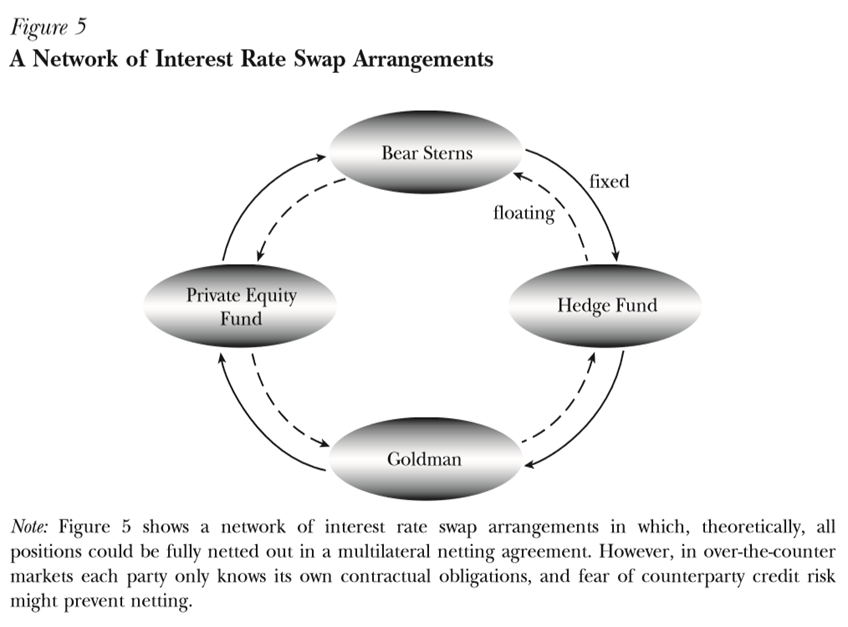
\includegraphics{Figures/swap_net_vs_gross.png}
}

\caption{\label{fig:L4_swap_net_vs_gross} Complexity and opacity of interbank and financial intermediary networks implies netting of positions subject to ambiguity. Source: \href{https://www.princeton.edu/~markus/research/papers/liquidity_credit_crunch.pdf}{Brunnermeier (2009); Bloomberg}}

\end{center}
\end{figure}

\end{frame}

%-------------------------------------------------------

%-------------------------------------------------------

\begin{frame}{Run on repo}

Remember Diamond-Dybvig model of bank runs and the famous movie, \emph{`It's a wonderful life'}\ldots

\end{frame}

%-------------------------------------------------------

%-------------------------------------------------------

\begin{frame}{Run on repo}

\begin{figure}
\begin{center}

\resizebox{0.70\textwidth}{!}{%
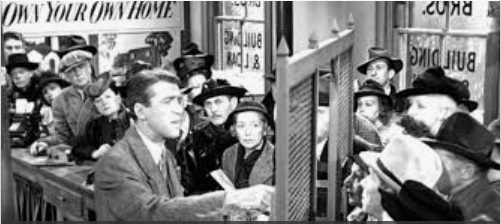
\includegraphics{Figures/its_wonderful.png}
}

\end{center}
\end{figure}

\end{frame}

%-------------------------------------------------------

%-------------------------------------------------------

\begin{frame}{Run on repo}

\ldots or \emph{`Mary Poppins'}\ldots

\end{frame}

%-------------------------------------------------------

%-------------------------------------------------------

\begin{frame}{Run on repo}

\begin{figure}
\begin{center}

\resizebox{0.70\textwidth}{!}{%
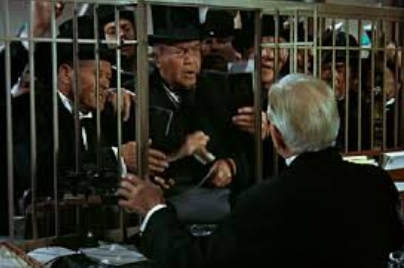
\includegraphics{Figures/mary_poppins_1.png}
}

\end{center}
\end{figure}

\end{frame}

%-------------------------------------------------------

%-------------------------------------------------------

\begin{frame}{Run on repo}

\begin{figure}
\begin{center}

\resizebox{0.70\textwidth}{!}{%
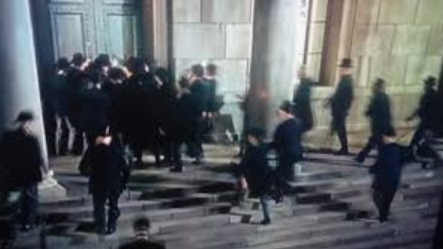
\includegraphics{Figures/mary_poppins_2.png}
}

\end{center}
\end{figure}

\end{frame}

%-------------------------------------------------------

%-------------------------------------------------------

\begin{frame}{Run on repo}

\begin{quote}
What happened is analogous to the banking panics of the 19th century in which depositors \emph{en masse} went to their banks seeking to withdraw cash in exchange of demand and savings deposits. \textbf{The banking system could not honor these demands because the cash had been lent out and the loans were illiquid}, so instead they suspended convertibility and relied on clearinghouses to issue certificates as makeshift currency. Evidence of the insolvency of the banking system in these earlier episodes is the discount on these certificates. \textbf{We argue that the current crisis is similar in that contagion led to `withdrawals' in the form of unprecedented high repo haircuts and even the cessation of repo lending on many forms of collateral.}
\end{quote}
\begin{center}
- Gorton and Metrick (2009)
\end{center}

\end{frame}

%-------------------------------------------------------

%-------------------------------------------------------

\begin{frame}{Run on repo}

Investor buys some asset (acts as collateral) from the bank for $X$
\begin{itemize}
\item	Bank agrees to repurchase the same asset some time later (perhaps the next
day) for $Y$
\item	The percentage (Y-X)/X is the “repo rate” ($\approx$ interest
rate on a bank deposit)
\item	Typically, the total amount of the deposit will be some amount less than the value of the underlying asset (the difference is the `haircut').
\end{itemize}
\vspace{2mm}
Numerical example\ldots
	\begin{itemize}
	\item	An asset has a market value of $100$
	\item	Bank sells it for $80$ with an agreement to repurchase it for $88$
	\item	Repo rate is $10\%$ $\left( \frac{88-80}{80} \right)$
	\item	Haircut is $20\%$ $\left( \frac{100 – 80}{100} \right)$
	\item	If bank defaults on promise to repurchase, the investor keeps collateral
	\end{itemize}

\end{frame}

%-------------------------------------------------------

%-------------------------------------------------------

\begin{frame}{Run on repo}

Pools of mortgages are used as collateral by SPVs when they borrow
\begin{itemize}
\item	Also, the outputs of securitization (MBS etc.) are \textit{themselves} often used as collateral
\end{itemize}
\vspace{2mm}
Haircut plays the role of reserves (covering a fraction of deposits) in the traditional model of banking
	\begin{itemize}
	\item	Forces bank to keep some fraction of their assets in reserve
	\item	Note this captures a form of `solvency' protection
	\end{itemize}
\vspace{2mm}
Collateral plays the role of (govt-provided) deposit insurance in traditional model of banking
\begin{itemize}
\item	Maintains faith of lender
\item	What what if collateral starts to be questioned?
\end{itemize}

\end{frame}

%-------------------------------------------------------

%-------------------------------------------------------

\begin{frame}{Run on repo}

\begin{figure}
\begin{center}

\resizebox{0.70\textwidth}{!}{%
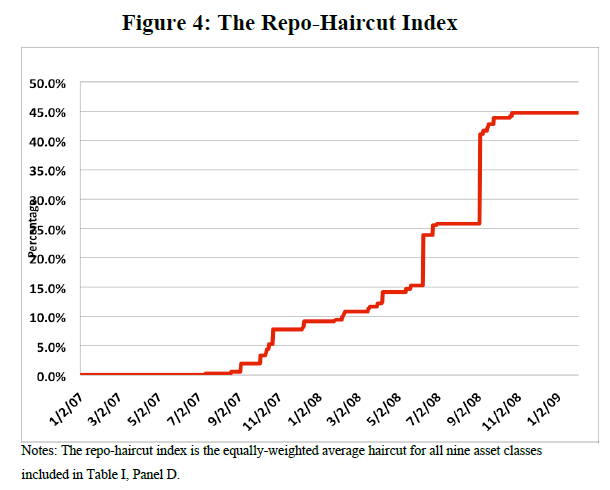
\includegraphics{Figures/gorton_metrick_repo_haircut.png}
}

\caption{\label{fig:L4_gorton_metrick_repo_haircut} Repo haircut - averaged over asset classes. Source: Gorton and Metrick (2009)}

\end{center}
\end{figure}

\end{frame}

%-------------------------------------------------------

%-------------------------------------------------------

\begin{frame}{Run on repo}

Numerical example of effects of haircut $\uparrow$
	\begin{itemize}
	\item	Suppose repo market size $= 10$
	\item	Haircut of $0\%$ $\Rightarrow$ banks can raise financing of $10$
	\item	Suppose haircut rises to $20\%$ on average
	\item	Then banks can only raise $8$ in financing
	\item	Need to find other ways - new securities? Difficult.
	\item	May need to sell assets - but this might drive prices down and will typically be the assets used as collateral!
	\item	This hampers them further as raises more concern about solvency - leading to higher haircuts\ldots
	\end{itemize}
\vspace{2mm}
Additionally, the size of the potential market might shrink
\begin{itemize}
\item	Money market funds leaving the market
\end{itemize}

\end{frame}

%-------------------------------------------------------

%-------------------------------------------------------

\begin{frame}{Crisis timeline}

There are useful timelines of the crisis online (I here summarize)
	\begin{itemize}
	\item	\href{https://www.stlouisfed.org/financial-crisis/full-timeline\#2008}{St Louis Fed}
	\item	\href{https://www.thebalance.com/2007-financial-crisis-overview-3306138}{2007}, \href{https://www.thebalance.com/2008-financial-crisis-timeline-3305540}{2008} and \href{https://www.thebalance.com/2009-financial-crisis-bailouts-3305539}{2009} from `The Balance' website
	\end{itemize}
\vspace{3mm}
See, also, the timelines provided in \href{https://www.princeton.edu/~markus/research/papers/liquidity_credit_crunch.pdf}{Brunnermeier (2009)} and, more recently, in \href{https://pubs.aeaweb.org/doi/pdfplus/10.1257/jep.33.1.107}{Aikman \emph{et al} (2019)}

\end{frame}

%-------------------------------------------------------

%-------------------------------------------------------

\begin{frame}{Crisis timeline - 2007}

\textbf{Early 2007}
	\begin{itemize}
	\item	Home sales/prices peak and troubles emerge in MBS and funds invested in them
	\item	New Century Financial `death spiral' (subprime lender), Bear Stearns suspended redemptions from a prominent fund, ratings downgrades on swathes of MBS
	\end{itemize}
\vspace{2mm}
\textbf{Summer}
	\begin{itemize}
	\item	Housing market numbers continued to worsen and, in late Summer, interbank lending was stressed (recall Ted spread discussion)
	\item	Fed cuts rate by 50bp in August to 4.75 (would be 4.25 by year-end)
	\item	American Home Mortgage Investment Corporation goes bankrupt
	\item	BNP Paribas halts redemptions on mortgage/MBS related funds
	\end{itemize}
\vspace{2mm}	
\textbf{Fall}
	\begin{itemize}
	\item	Housing market continues to weaken
	\item	Northern Rock (old-skool) run in the UK
	\end{itemize}

\end{frame}

%-------------------------------------------------------

%-------------------------------------------------------

\begin{frame}{Crisis timeline - 2007}

\textbf{December}
	\begin{itemize}
	\item	Transmission of monetary policy (rate cuts) was not freeing up bank lending as spreads over safe rates were widening
	\item	To avoid stigma of discount window lending, Fed creates Term Auction Facility
		\begin{itemize}
		\item	Provides collateralized (even with various MBS) funding to banks with sub-prime exposures
		\item	Trying to follow Bagehot approach
		\item	Like an anonymous discount window
		\item	Intended to give breathing room - avoid firesale into closed/dislocated markets
		\end{itemize}
	\item	Foreclosures pick up speed - but problems still largely restricted to financial markets, banking system and housing market (not broader economy, yet)
	\end{itemize}

\end{frame}

%-------------------------------------------------------

%-------------------------------------------------------

\begin{frame}{Crisis timeline - 2007}

\begin{quote}
Under the Term Auction Facility (TAF) program, the Federal Reserve will auction term funds to depository institutions against the wide variety of collateral that can be used to secure loans at the discount window.  All depository institutions that are judged to be in generally sound financial condition by their local Reserve Bank and that are eligible to borrow under the primary credit discount window program will be eligible to participate in TAF auctions.  All advances must be fully collateralized.  By allowing the Federal Reserve to inject term funds through a broader range of counterparties and against a broader range of collateral than open market operations, this facility could help promote the efficient dissemination of liquidity when the unsecured interbank markets are under stress.
\end{quote}

\end{frame}

%-------------------------------------------------------

%-------------------------------------------------------

\begin{frame}{Crisis timeline - 2008}

\textbf{Early 2008}
	\begin{itemize}
	\item	Fed continues cutting
	\item	Tax rebates announced (though not to be paid until summer)
	\item	But housing market and foreclosures keep worsening
	\item	BoA buys Countrywide (aggressive subprime lender) and Ambac Financial Group downgraded (important guarantor / monoline insurer)
	\end{itemize}
\vspace{2mm}
\textbf{March}
	\begin{itemize}
	\item	Fed extends TAF and other lending facilities
		\begin{itemize}
		%\item	Provide banks holding MBS and CDOs with `good' assets collateral they could then use for funding
		\item	\textbf{Note these are liquidity policies}
		\end{itemize}
	\item	Bear `failure' - acquisition by J. P. Morgan Chase
		\begin{itemize}
		\item	JPMC agreed to pay \$2 a share ($<7\%$ of price two days earlier)
		\item	Partly backed by Fed but JPMC had a first loss position (junior loan)
		\end{itemize}
	\item	Loosening by Fed and opened discount window to investment banks via `Primary Dealer Credit Facility'
		\begin{itemize}
		\item	Overnight funding to investment banks
		\item	Helped Lehman, for now\ldots
		\end{itemize}
	\end{itemize}

\end{frame}

%-------------------------------------------------------

%-------------------------------------------------------

\begin{frame}{Crisis timeline - 2008}

\textbf{Spring-Summer}
	\begin{itemize}
	\item	Further emergency lending by Fed
	\item	Indymac failure
	\item	Housing and Economic Recovery Act allowed Treasure to guarantee some loans backed by Fannie and Freddie (GSEs that securitized huge fraction of U.S. mortgages)
	\item	Discussions about possible future support for the GSEs
	\end{itemize}

\textbf{September}
	\begin{itemize}
	\item	Fannie and Freddie put into conservatorship
		\begin{itemize}
		\item	Made explicit and formalized government backing of the GSEs that had previously been assumed (allowed them to be aggressive in expansion)
		\item	\textbf{Note the similarity to deposit insurance and other moral hazard examples}
		\end{itemize}
	\item	Lehman Brothers failure
		\begin{itemize}
		\item	Had been an attempt to form a private sector buyout
		\item	But Korean SWF, Barclays and BoA backed off (BoA buys Merrill)
		\item	Debate over why Fed `allowed' Lehman to fail\ldots
		\end{itemize}
	\end{itemize}

\end{frame}

%-------------------------------------------------------

%-------------------------------------------------------

\begin{frame}{Crisis timeline - 2008}

Brief aside on Lehman failure
	\begin{itemize}
	\item	Highly levered (less restricted by regulation since not depository institution)
	\item	Short term funding
	\item	Highly exposed to housing market directly and through complex derivatives/MBS
	\item	Had to take big write-downs - especially in subprime (weakening capital position)
	\item	Tried to delever and raise funding but opacity of assets and suspicion in market hindered this
	\item	Once private sector bailout failed and (according to the Fed) it was decided that Lehman had inadequate collateral to secure a loan from the Fed with sufficient certainty that the Fed would not take a loss
	\end{itemize}

\end{frame}

%-------------------------------------------------------

%-------------------------------------------------------

\begin{frame}{Crisis timeline - 2008}

Ball (2018) argues that the Fed's claim that they could not legally provide a loan, was false and not the real reason
	\begin{itemize}
	\item	Implies it was a political decision to avoid moral hazard (driven by Paulson)
	\item	Claims there were plenty of assets that, even conservatively valued, could have secured a loan to allow at least an orderly wind-down (avoiding value destruction that certainly did occur in the chaos)
	\item	Should have helped as they helped Bear and, soon after, helped AIG
	\item	Hadn't realized that the effects would be so disruptive (Bernanke strongly disagrees)
	\end{itemize}
\end{frame}

%-------------------------------------------------------

%-------------------------------------------------------

\begin{frame}{Crisis timeline - 2008}

Great reference to understand `How big banks fail' is Duffie's book of that title
\begin{itemize}
\item	Here I quickly summarize his description of the stages of a `typical' failure (of a big dealer bank - see Bear, Lehman)
\item	This and the (more difficult) Ball book are very useful for getting a grip on the nuts and bolts of how these banks functioned before the crisis (without endorsing Ball's take on why Lehman was `allowed' to fail)
\item	You won't be tested on minute details of these books - but they're good reads if you're interested in this world\ldots
\end{itemize}

\end{frame}

%-------------------------------------------------------

%-------------------------------------------------------

\begin{frame}{How a big bank fails}


\begin{quote}
Dealer banks are financial institutions that intermediate the `backbone' markets for securities and over-the-counter (OTC) derivatives. These activities tend to be bundled with other
wholesale financial market services, such as prime brokerage and underwriting. Because of
their size and their central position in the plumbing of the financial system, the failure of
a dealer bank could place significant stress on its counterparties and clients, and also on
the prices of assets or derivatives that it holds. The collapse of a major dealer bank also
reduces the ability of the financial system to absorb further losses and to provide credit and
liquidity to major market participants. Thus, the potential failure of a major dealer bank is
a systemic risk.
\end{quote}
\begin{center}
- Duffie, \emph{How big banks fail - and what to do about it}, 2011
\end{center}

\end{frame}

%-------------------------------------------------------

%-------------------------------------------------------

\begin{frame}{How big banks fail}

\begin{figure}
\begin{center}

\resizebox{0.90\textwidth}{!}{%
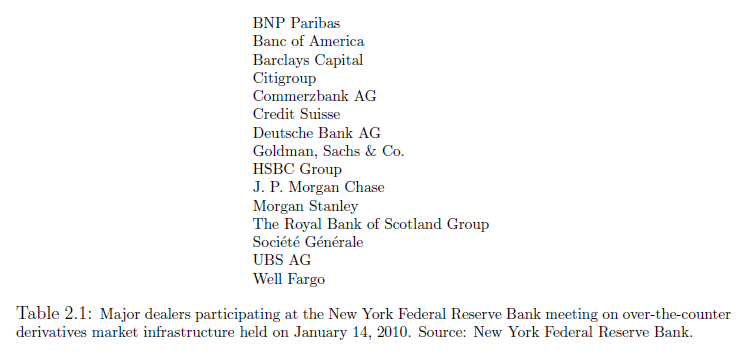
\includegraphics{Figures/dealer_banks.png}
}

\end{center}
\end{figure}

\end{frame}

%-------------------------------------------------------

%-------------------------------------------------------

\begin{frame}{How a big bank fails}

Suppose something (MBS?) has happened to cause substantial losses or drains on liquidity for bank, `Beta'
	\begin{itemize}
	\item	Hasn't devastated the bank but has weakened its position notably	
	\end{itemize}
\vspace{2mm}
Bank tries to signal strength and protect franchise value by not scaling back, but `putting on a brave face'
	\begin{itemize}
	\item	To prevent loss of counterparties and clients they bail out clients on investments arranged by Beta and continue to offer them good terms (e.g. implicit backing for off balance sheet SPVs)
	\item	But this drains funds (which in the future will be a problem)
	\end{itemize}


\end{frame}

%-------------------------------------------------------

%-------------------------------------------------------

\begin{frame}{How a big bank fails}

Confidence dented $\Rightarrow$ counterparties are avoiding Beta/reducing positions
	\begin{itemize}
	\item	Might need to top up their collateral / satisfy margin calls
	\item	Other dealers may be asked to step in between Beta and its counterparties (novations)
	\item	Rumours spread as dealers become wary of increasing \emph{their} positions
	\end{itemize}
\vspace{0.5mm}
Beta also has a prime-brokerage business for hedge fund clients, say
	\begin{itemize}
	\item	Provides IT, trade execution, accounting reports
	\item	Vitally, also custodian services - keeps the HF's cash and securities
	\item	HF start to ask for them back to shift them to other dealers
	\item	Can't really say no or rumours become a clamour
	\item	Damages franchise value (this was profitable) eroding attractiveness for investors further - vicious circle
	\item	Note also, the HF securities were frequently used by Beta \emph{on its own behalf} in repo borrowing as collateral - so double/triple whammy
	\end{itemize}

\end{frame}

%-------------------------------------------------------

%-------------------------------------------------------

\begin{frame}{How a big bank fails}

Even \textit{secured} creditors start backing away (disaster)
	\begin{itemize}
	\item	Even if collateral is thought solid, why bother getting involved in admin around default?
	\item	They themselves may need funds and collateral back quickly
	\item	Haircuts also might no longer be though adequate (will they be able to sell collateral for enough even if they get it back?)
	\end{itemize}
\vspace{2mm}
A lot of these loans are repo (recall Gorton) and \textbf{a lot} is rolled over every night
	\begin{itemize}
	\item	If reluctance to lend occurs, the impacts are rapid (recall our discussion last week of shortening of maturity of debt, pre-crisis)
	\item	Must find a lot more funding - especially as haircuts are rising
	\item	Or start selling - but assets are opaque and possibly already underpriced!
	\end{itemize}

\end{frame}

%-------------------------------------------------------

%-------------------------------------------------------

\begin{frame}{How a big bank fails}

Banks need to hold enough cash/securities in clearing accounts
	\begin{itemize}
	\item	Usually only need to average out over the day - intraday credit from clearing banks
	\item	But clearing banks don't want to be left holding the can either
	\item	Removal of intraday credit is the endgame
	\item	Can't execute trades - dead\ldots
	\item	Declare bankruptcy
	\end{itemize}
\end{frame}

%-------------------------------------------------------

%-------------------------------------------------------

\begin{frame}{How big banks fail}

\begin{figure}
\begin{center}

\resizebox{0.60\textwidth}{!}{%
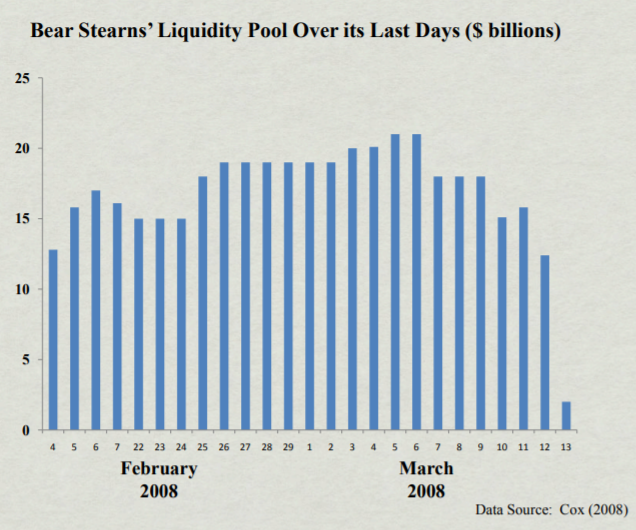
\includegraphics{Figures/bear_stearns_liquidity.png}
}

\end{center}
\end{figure}

\end{frame}

%-------------------------------------------------------

%-------------------------------------------------------

\begin{frame}{Crisis timeline - 2008}

\textbf{Back to September 2008}
	\begin{itemize}
	\item[]	Fed buys AIG
		\begin{itemize}
		\item	Had used their profitable \emph{core} insurance business to fund a business insuring mortgage/mortgage derivative positions - including insuring securities
		\item	Was hugely interconnected via this insurance
		\item	If they failed, the insurance would vanish, causing huge losses across swathes of investors and further asset price declines
		\item	AIG avoided a disruptive bankruptcy but shareholders were wiped out and replaced with Treasury preferred shares etc. after Fed initially made loans (contrast with Lehman)
		\end{itemize}
	\end{itemize}

\end{frame}

%-------------------------------------------------------

%-------------------------------------------------------

\begin{frame}{Crisis timeline - 2008}

\textbf{Still September 2008 - not a good month}
	\begin{itemize}
	\item[]	Reserve Primary Fund broke the buck and broader MMF problems
		\begin{itemize}
		\item	Partly from direct exposure to Lehman (RPF) - also from general contagion and concern at their holdings
		\item	\textbf{Any sniff of risk in these funds and depositors would pull out (they had previously been thought to be riskless - like money)}
		\item	\textcolor{red}{\textbf{MMF unable to finance themselves would pull back on CP holdings which is lifeblood of corp America for working capital}}
		\item	Fed insurance of MMF via `Asset-backed CP MMF Liquidity Facility'
		\end{itemize}
\vspace{1mm}
\item[]	Goldman and MS become commercial banks
	\begin{itemize}
	\item	Can access discount window
	\item	\textbf{No more investment banks on Wall Street!}
	\end{itemize}
\vspace{1mm}
\item[]	WaMu bankrupt after `silent' run
	\begin{itemize}
	\item	Handled by FDIC and sold to JPMC
	\item	Also, Wachovia bought by Wells
	\end{itemize}
\vspace{1mm}
\item[]	Treasury requests $\$700bn$ fund from Congress
	\begin{itemize}
	\item	Defeated despite protections for taxpayer and restrictions on banks
	\item	DJ plunges 770 points
	\end{itemize}
	\end{itemize}

\end{frame}

%-------------------------------------------------------

%-------------------------------------------------------

\begin{frame}{Crisis timeline - 2008}

\textbf{Autumn}
	\begin{itemize}
	\item[]	Bill eventually passed on second attempt
		\begin{itemize}
		\item	Emergency Economic Stabilization Act
		\item	Funded `Troubled Asset Relief Program' (TARP)\ldots
		\item	Helped with Capital Purchase Program (injecting funds into banks with stock purchases - i.e. `bailouts' though doesn't imply a loss for taxpayer)
		\item	Additionally - used for AIG, autos companies, `Term Asset-Backed Securities Loan Facility (TALF) and some homeowner refi programs
		\item	Bill also increased salary oversight (surprisingly effective), FDIC insurance limit and suspended some mark to market accounting requirements (response to firesales)
		\end{itemize}
	\vspace{2mm}
	\item[]	Wheels started to come off stock markets around the world
		\begin{itemize}
		\item	Coordinated rate cuts by central banks in response (\textbf{rapidly approaching ZLB})
		\end{itemize}
	\vspace{2mm}
	\item[]	Fed started `Commerical Paper Funding Facility'
		\begin{itemize}
		\item	Buying commerical paper from \textit{highly rated} firms (\textit{even they} couldn't access CP markets)
		\end{itemize}
	\end{itemize}
	
\end{frame}

%-------------------------------------------------------

%-------------------------------------------------------

\begin{frame}{Crisis timeline - 2008}

\textbf{Autumn}
	\begin{itemize}
	\item	Fed set up Money Market Investor Funding Facility
		\begin{itemize}
		\item	To take assets off money market funds and lend them sums to deal with redemptions
		\end{itemize}
	\vspace{2mm}
	\item	Citi receives funding injections
	\vspace{2mm}
	\item	Fed cuts rates to zero
	\vspace{2mm}
	\item	TALF bought debt of non-mortgage securitizers
		\begin{itemize}
		\item	Credit cards, autos, student loans\ldots
		\item	\textbf{Fear of anything securitized had spread!}
		\end{itemize}
	\end{itemize}

\end{frame}

%-------------------------------------------------------

%-------------------------------------------------------

\begin{frame}{Crisis timeline - 2009}

\textbf{February}
	\begin{itemize}
	\item[]	$\$787bn$ economic stimulus package under Obama
		\begin{itemize}
		\item	Homeowner Stability Initiative also launched to help prevent foreclosure
		\item	Revealed that GDP growth was $-6.3\%$ at end of 2008
		\end{itemize}
	\end{itemize}
\vspace{1mm}
\textbf{April}
	\begin{itemize}
	\item[]	Homeowner Affordable Mortgage Program (HARP
		\begin{itemize}
		\item	To promote financing for underwater borrowers
		\item	Rates had fallen but negative equity prevented taking out new mortgages / refi to access them
		\item	Low takeup - by people only slightly underwater - foreclosures continue
		\end{itemize}
	\end{itemize}
\vspace{1mm}
\textbf{October}
	\begin{itemize}
	\item	Unemployment rate reaches $10\%$
	\item	Lending down - loan performance also
	\item	Banks trying to rebuild balance sheets - cuts off credit
	\item	Households trying to rebuild balance sheets - demand declines
	\end{itemize}

\end{frame}

%-------------------------------------------------------

%-------------------------------------------------------

\begin{frame}{Broader effects of the crisis}

So far we've mainly focused on the financial aspects of the crisis
\begin{itemize}
\item	Ultimately, the effect on the broader economy is the most important motivation for reform
\item	We cannot give a complete analysis here
\item	Some of the main channels discussed are\ldots
	\begin{itemize}
	\item	Traditional accelerationist channels through bank weakness and financial market panic
		\begin{itemize}
		\item	Emphasized in Bernanke (2018) in reading list
		\end{itemize}
	\item	Household leverage/debt channel
		\begin{itemize}
		\item	Emphasized by Mian and Sufi (various papers and book)
		\end{itemize}
	\item	Fiscal damage 
		\begin{itemize}
		\item	See recent work by Oscar Jorda \emph{et al}
		\end{itemize}
	\end{itemize}
\end{itemize}

\end{frame}

%-------------------------------------------------------

%-------------------------------------------------------

\begin{frame}{Economic impacts - Housing market}

\begin{figure}
\begin{center}

\resizebox{0.80\textwidth}{!}{%
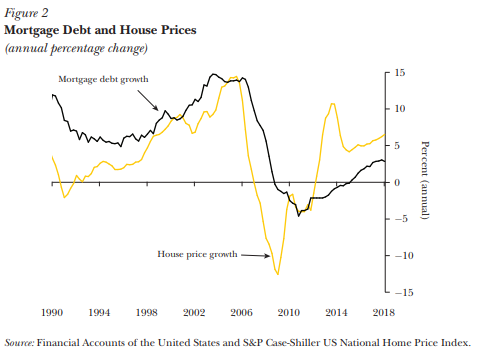
\includegraphics{Figures/aikman_et_al_house_prices_mortage.png}
}

\caption{House prices and mortgage debt. Source: \href{https://pubs.aeaweb.org/doi/pdfplus/10.1257/jep.33.1.107}{Aikman \emph{et al} (2019)}}

\end{center}
\end{figure}

\end{frame}

%-------------------------------------------------------

%-------------------------------------------------------

\begin{frame}{Economic impacts - Household credit problems}

\begin{figure}
\begin{center}

\resizebox{0.80\textwidth}{!}{%
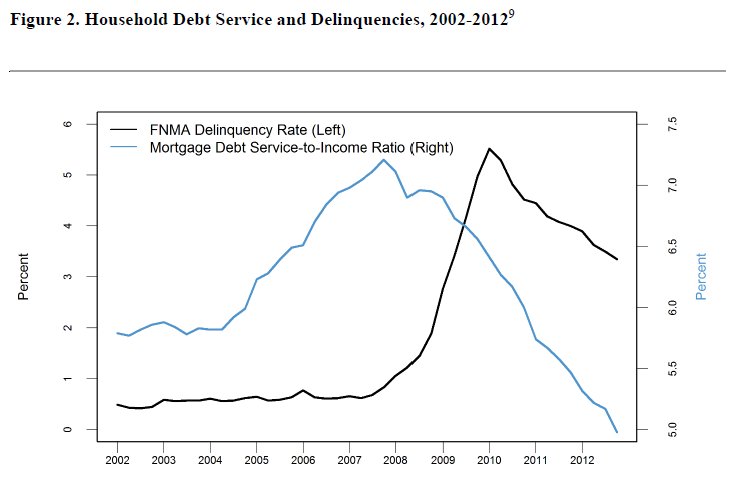
\includegraphics{Figures/dti_and_delinquencies.png}
}

\caption{Household debt to income and delinquencies. Source: Bernanke (2018)}

\end{center}
\end{figure}

\end{frame}

%-------------------------------------------------------

%-------------------------------------------------------

\begin{frame}{Economic impacts - Corporate credit problems}

\begin{figure}
\begin{center}

\resizebox{0.80\textwidth}{!}{%
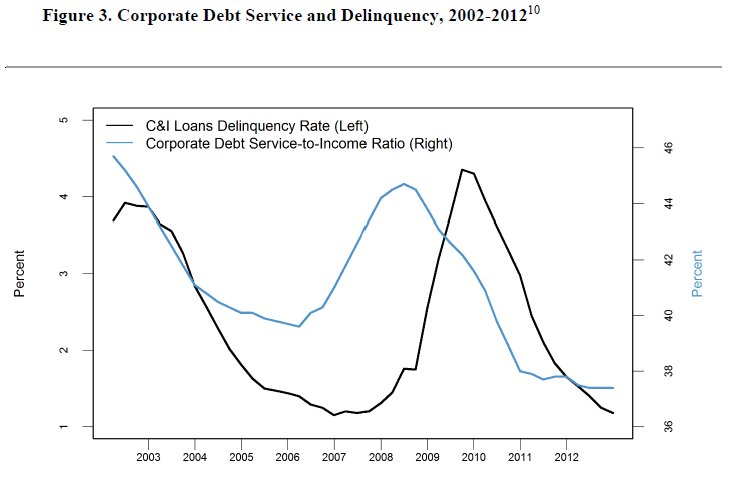
\includegraphics{Figures/corp_loans_delinquency.png}
}

\caption{Corporate debt servicing and delinquencies. Source: Bernanke (2018)}

\end{center}
\end{figure}

\end{frame}

%-------------------------------------------------------

%-------------------------------------------------------

\begin{frame}{Economic impacts - Labor market problems}

\begin{figure}
\begin{center}

\resizebox{0.90\textwidth}{!}{%
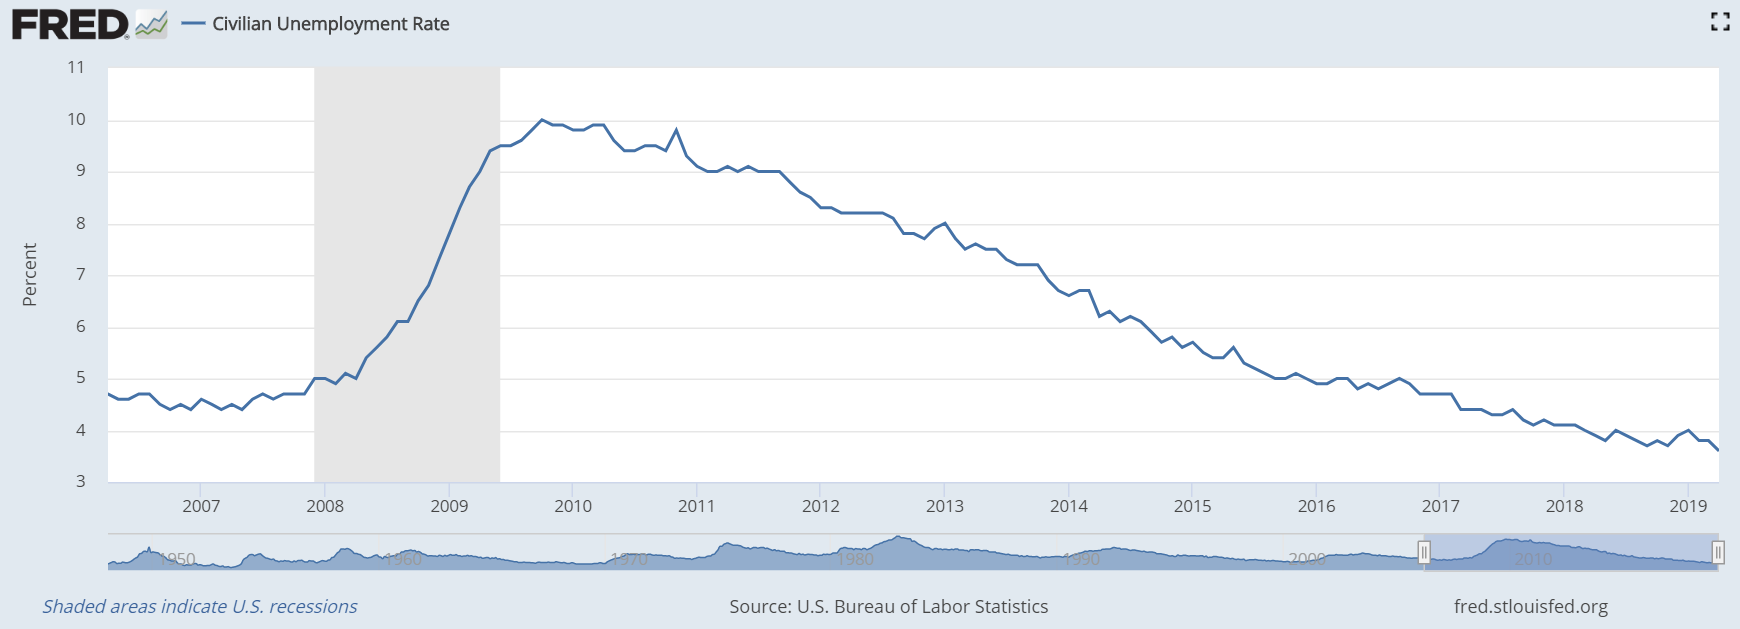
\includegraphics{Figures/unemployment_rate.png}
}

\caption{Unemployment rate. Source: FRED}

\end{center}
\end{figure}

\end{frame}

%-------------------------------------------------------

%-------------------------------------------------------

\begin{frame}{Economic impacts - Deep recession}

\begin{figure}
\begin{center}

\resizebox{0.90\textwidth}{!}{%
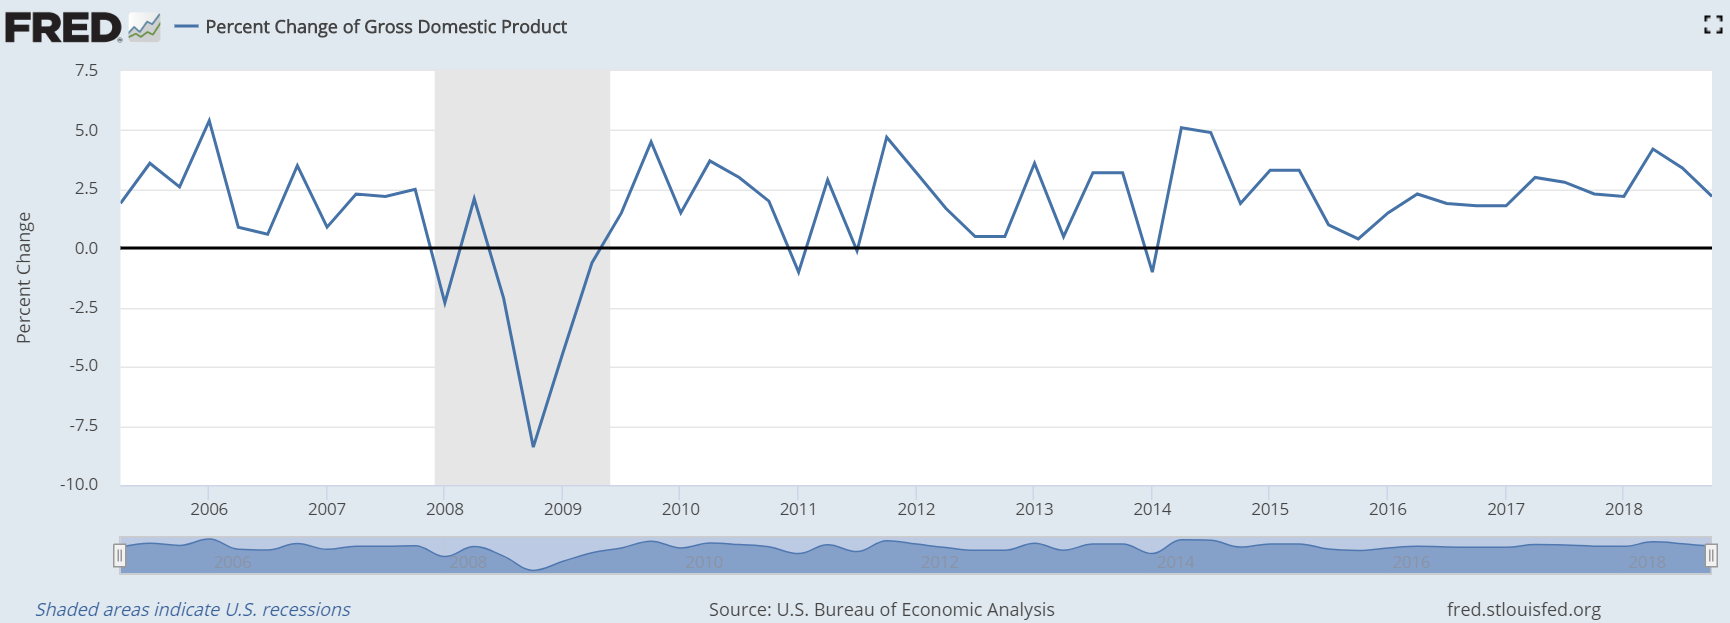
\includegraphics{Figures/recession.png}
}

\caption{Percentage growth in GDP. Source: FRED}

\end{center}
\end{figure}

\end{frame}

%-------------------------------------------------------

%-------------------------------------------------------

\begin{frame}{Economic impacts - Investment off a cliff}

\begin{figure}
\begin{center}

\resizebox{0.90\textwidth}{!}{%
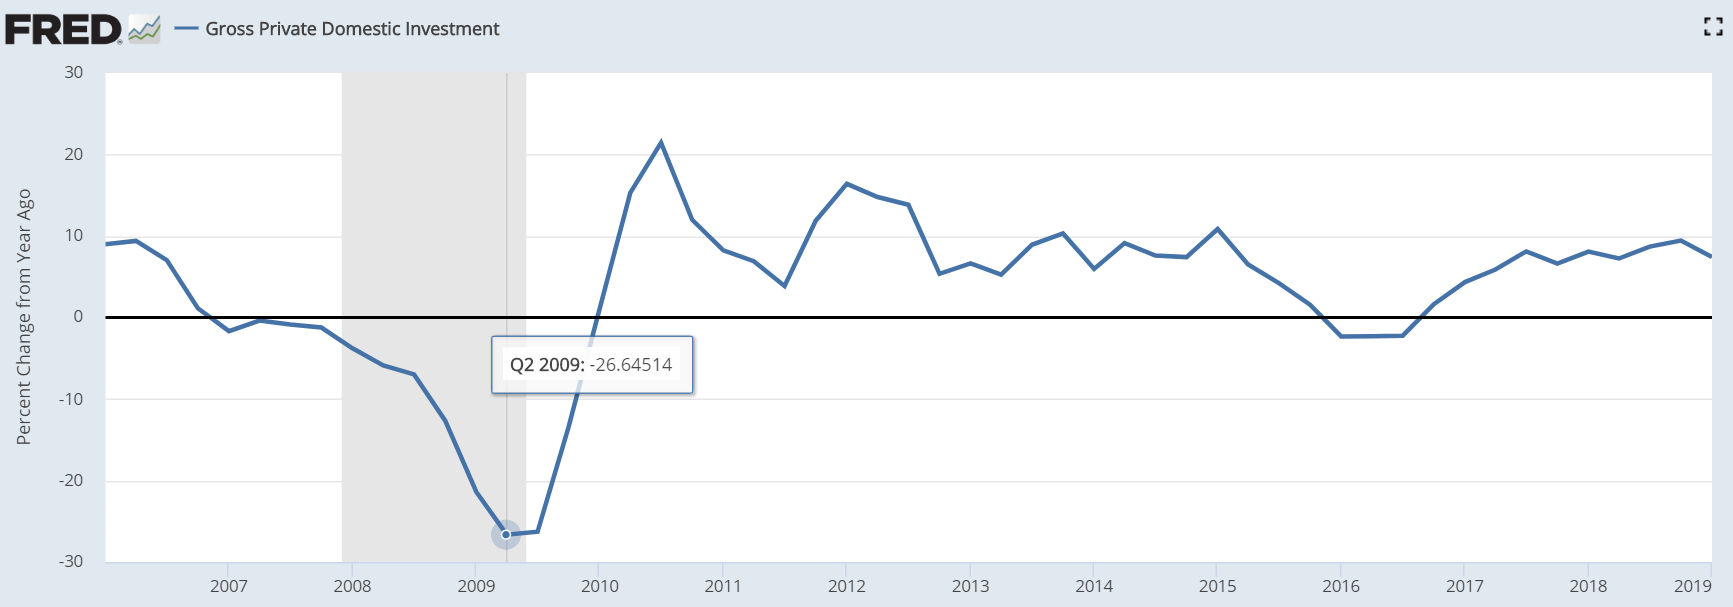
\includegraphics{Figures/investment.png}
}

\caption{Percentage growth YoY in Gross Private Domestic Investment. Source: FRED}

\end{center}
\end{figure}

\end{frame}

%-------------------------------------------------------

%-------------------------------------------------------

\begin{frame}{Economic impacts - Some feedbacks to banks}

\begin{figure}
\begin{center}

\resizebox{0.80\textwidth}{!}{%
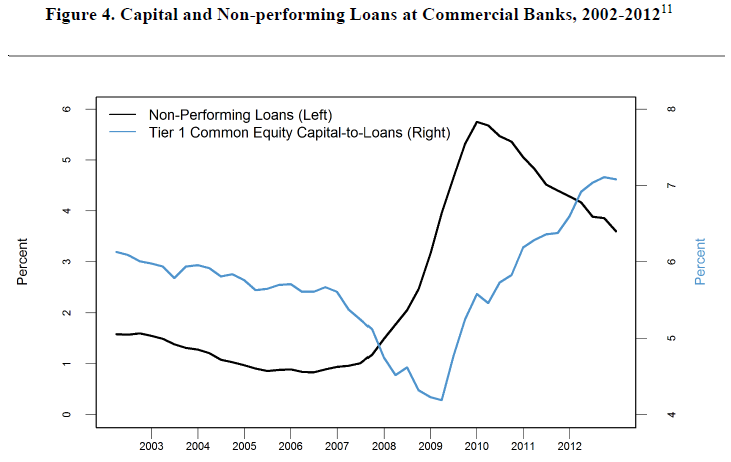
\includegraphics{Figures/npl_commercial_banks.png}
}

\caption{Bad loans grind down bank equity. Source: Bernanke (2018)}

\end{center}
\end{figure}

\end{frame}

%-------------------------------------------------------

%-------------------------------------------------------

\begin{frame}{Broader effects of the crisis}

In the work of Jorda \emph{et al} (various papers) they emphasize that
	\begin{itemize}
	\item	Recessions after \textit{financial} crises are often more prolonged and severe
	\item	A preceding credit bubble is particularly damaging
	\item	Pre-crisis fiscal strength can help mitigate the effects
	\end{itemize}

\end{frame}

%-------------------------------------------------------

%-------------------------------------------------------

\begin{frame}{Slow recovery from Great Recession}

\begin{figure}
\begin{center}

\resizebox{0.65\textwidth}{!}{%
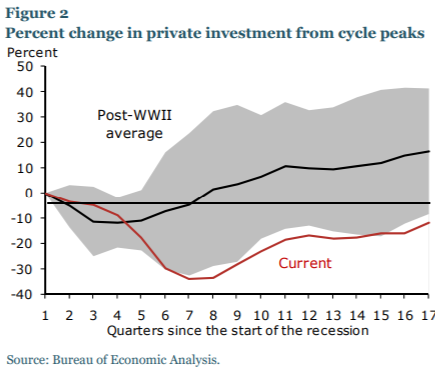
\includegraphics{Figures/investment_av_rec_and_most_recent.png}
}

\caption{Comparing recent and average recovery in investment. Source: Jorda (2012)}

\end{center}
\end{figure}

\end{frame}

%-------------------------------------------------------

%-------------------------------------------------------

\begin{frame}{Slow recovery from Great Recession}

\begin{figure}
\begin{center}

\resizebox{0.65\textwidth}{!}{%
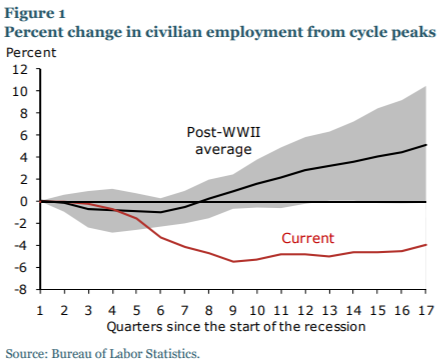
\includegraphics{Figures/unemp_av_rec_and_most_recent.png}
}

\caption{Comparing recent and average recovery in unemployment. Source: Jorda (2012)}

\end{center}
\end{figure}

\end{frame}

%-------------------------------------------------------

%-------------------------------------------------------

\begin{frame}{Fits pattern of recoveries from `financial' recessions}

\begin{figure}
\begin{center}

\resizebox{0.65\textwidth}{!}{%
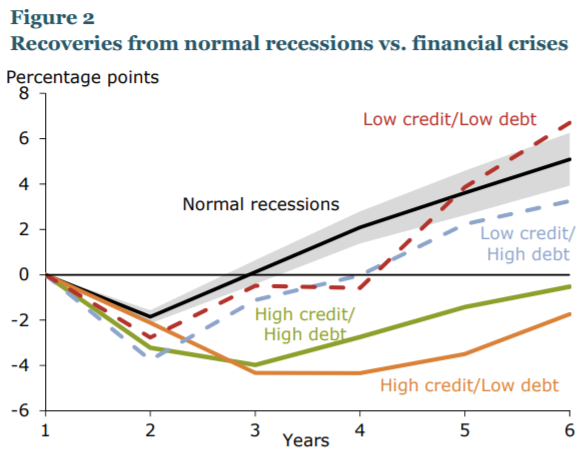
\includegraphics{Figures/recoveries_normal_rec_vs_fin_crises.png}
}

\caption{Comparing recoveries after `normal' and `financial' recessions. Source: Jorda (2012)}

\end{center}
\end{figure}

\end{frame}

%-------------------------------------------------------

%-------------------------------------------------------

\begin{frame}{Importance of public debt}

\begin{figure}
\begin{center}

\resizebox{0.65\textwidth}{!}{%
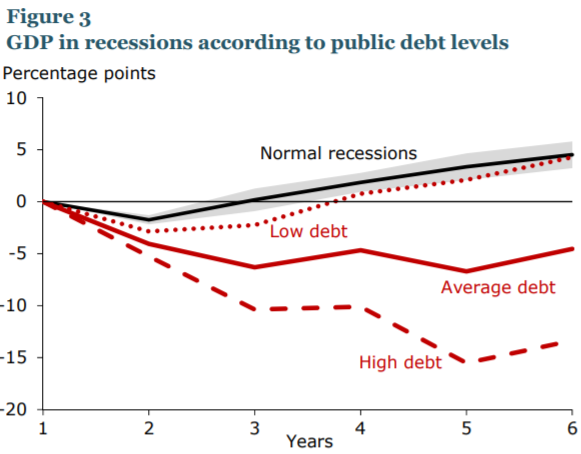
\includegraphics{Figures/recoveries_dependent_on_debt.png}
}

\caption{Comparing recoveries based on initial public debt. Source: Jorda (2012)}

\end{center}
\end{figure}

\end{frame}

%-------------------------------------------------------

%-------------------------------------------------------

\begin{frame}{Economic impacts - GFC damaged fiscal positions}

\begin{figure}
\begin{center}

\resizebox{0.90\textwidth}{!}{%
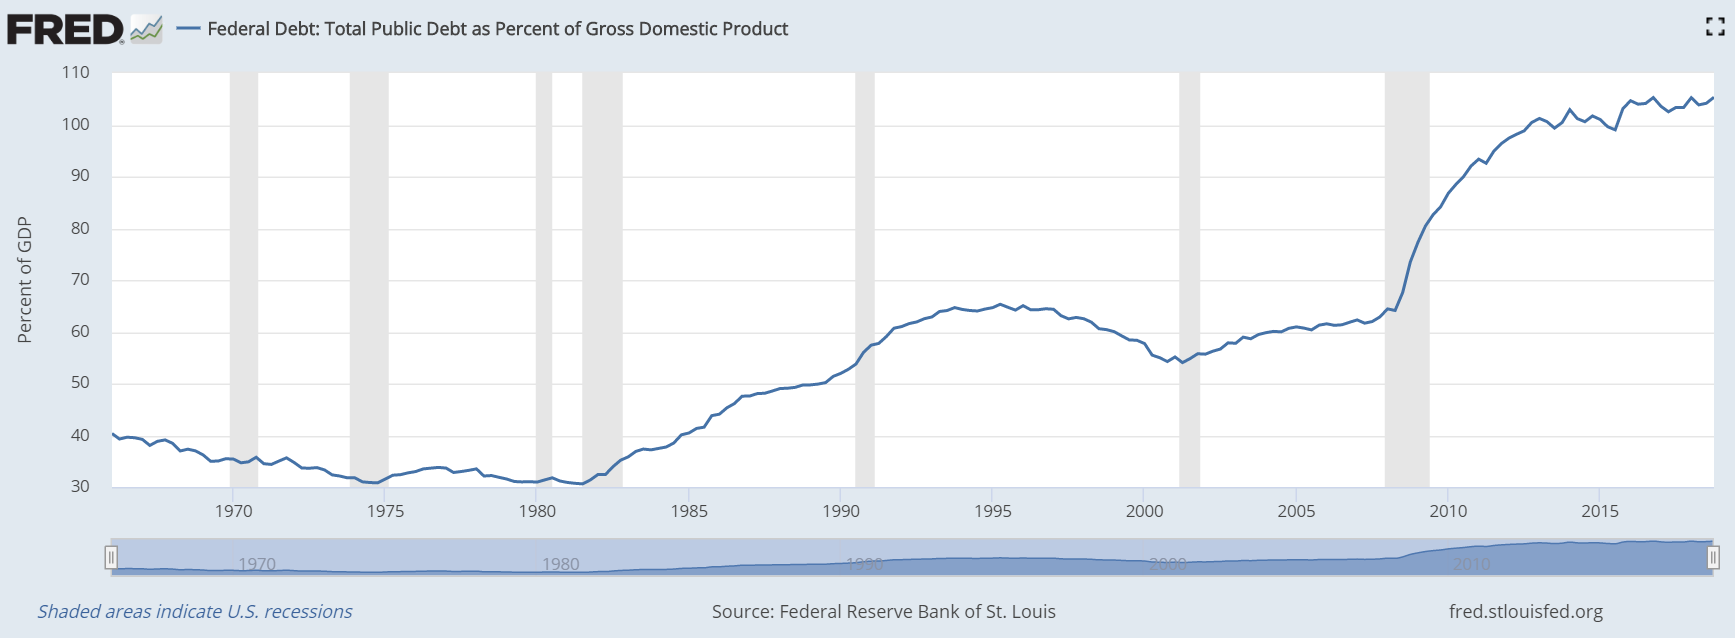
\includegraphics{Figures/debt_to_gdp_US.png}
}

\caption{Dramatic effect on debt levels. Source: FRED}

\end{center}
\end{figure}

\end{frame}

%-------------------------------------------------------

%-------------------------------------------------------

\begin{frame}{Some implications of fiscal damage}

We have concentrated on the US in this section
\begin{itemize}
\item	But the crisis was global
\item	Fiscal damage was widespread, putting, in some cases, immediate restrictions on countercyclical policy or bailouts
	\begin{itemize}
	\item	In some countries banks were both `too big to fail' \textbf{and} too big to save
	\item	Inadequate borrowing ability of governments necessitated austerity
	\item	Even in the U.S. many would argue the large stimulus bill under Obama should have been larger/continued longer
	\end{itemize}
\end{itemize}
\vspace{2mm}
Longer term, it may also imply important reductions in policy flexibility in the `next recession'\ldots
\begin{itemize}
\item	We're still close to ZLB and people question if QE effective
\item	Will fiscal policy be able to step in?
\end{itemize}

\end{frame}

%-------------------------------------------------------

%-------------------------------------------------------

\begin{frame}{But fiscal policy may not be available\ldots}

Ideally, a fiscal expansion can shift the `IS curve' to offset weakness
\begin{itemize}
\item	But, given the damage to fiscal position from GFC and ongoing issues with funding other excessively generous entitlements, will policymakers have enough firepower in the future?
\vspace{3mm}
\end{itemize}
\vspace{2mm}
Might need to rely on unconventional monetary policy and emergency measures again
	\begin{itemize}
	\item	But still controversial and poorly understood
	\item	Legal changes have also tied the Fed's hands in terms of crisis response
	\end{itemize}
\vspace{2mm}
Tricky time for the world economy
\begin{itemize}
\item	Good time for research / new thinking
\item	Go forth\ldots
\end{itemize}

\end{frame}


%\input{L_6_Post_crisis}

\end{document}
